\documentclass[12pt,a4paper]{article}

%% ── Packages ──────────────────────────────────────────────────────────────
\usepackage[T1]{fontenc}
\usepackage[utf8]{inputenc}
\usepackage{amsmath,amssymb,amsthm}
\usepackage{mathtools}
\usepackage{geometry}
\usepackage{graphicx}
\usepackage{xcolor}
\usepackage{booktabs}
\usepackage{array}
\usepackage{enumitem}
\usepackage{hyperref}
\usepackage{cleveref}
\usepackage{natbib}
\usepackage{setspace}
\usepackage{titlesec}
\usepackage{abstract}
\usepackage{epigraph}
\usepackage{tcolorbox}
\usepackage{pgfplots}
\pgfplotsset{compat=1.18}
\usepackage{tikz}
\usetikzlibrary{arrows.meta,positioning,decorations.pathreplacing}

%% ── Layout ────────────────────────────────────────────────────────────────
\geometry{left=3cm,right=3cm,top=3cm,bottom=3cm}
\onehalfspacing

%% ── Colours ───────────────────────────────────────────────────────────────
\definecolor{deepblue}{RGB}{0,51,102}
\definecolor{warmgray}{RGB}{245,242,238}
\definecolor{accent}{RGB}{180,50,30}

%% ── Hyperref ──────────────────────────────────────────────────────────────
\hypersetup{
  colorlinks=true,
  linkcolor=deepblue,
  citecolor=accent,
  urlcolor=deepblue,
  pdftitle={The Ecology of Neoteny},
  pdfauthor={Flyxion}
}

%% ── Section formatting ────────────────────────────────────────────────────
\titleformat{\section}{\large\bfseries\color{deepblue}}{\thesection.}{0.5em}{}
\titleformat{\subsection}{\normalsize\bfseries\color{deepblue}}{\thesubsection.}{0.5em}{}

%% ── Theorem environments ──────────────────────────────────────────────────
\theoremstyle{definition}
\newtheorem{definition}{Definition}[section]
\newtheorem{proposition}{Proposition}[section]
\newtheorem{corollary}{Corollary}[section]
\newtheorem{remark}{Remark}[section]

%% ── Operators ─────────────────────────────────────────────────────────────
\DeclareMathOperator{\Ent}{Ent}
\DeclareMathOperator{\diag}{diag}
\newcommand{\ddt}[1]{\frac{\mathrm{d}#1}{\mathrm{d}t}}
\newcommand{\ddx}[1]{\frac{\mathrm{d}#1}{\mathrm{d}x}}
\newcommand{\R}{\mathbb{R}}
\newcommand{\N}{\mathbb{N}}

%% ── Highlighted box ───────────────────────────────────────────────────────
\tcbset{
  policybox/.style={
    colback=warmgray, colframe=deepblue,
    fonttitle=\bfseries, title={Policy Implication},
    arc=2mm, boxrule=0.6pt, left=4pt, right=4pt, top=4pt, bottom=4pt
  },
  formalbox/.style={
    colback=warmgray, colframe=accent,
    fonttitle=\bfseries,
    arc=2mm, boxrule=0.6pt, left=4pt, right=4pt, top=4pt, bottom=4pt
  }
}

%% ══════════════════════════════════════════════════════════════════════════
\begin{document}

\begin{titlepage}
  \centering
  \vspace*{2cm}
  {\Huge\bfseries\color{deepblue} The Ecology of Neoteny\par}
  \vspace{0.4cm}
  {\large\itshape Institutions, Entropy, and the Steady-State Civilisation\par}
  \vspace{1.5cm}
  {\large Flyxion\par}
  \vspace{0.5cm}
  {\normalsize November 2025\par}
  \vspace{2cm}
  \hrule height 0.5pt
  \vspace{0.5cm}
  \begin{abstract}
    \noindent This essay argues that civilisation's creative longevity depends on the
    managed preservation of neotenous cognition---curiosity, play, and
    exploration---within protective institutional niches.  Drawing on Alison
    Gopnik's tripartite model of human intelligences (Exploit, Explore,
    Empower)~\citep{gopnik2016,gopnik2025}, it extends these ideas into an
    entropic framework, treating curiosity as a thermodynamic variable that must
    be subsidised and regulated.  The result is a vision of the
    \emph{steady-state civilisation}---a society that sustains perpetual
    exploration through equilibrium, not expansion.  Empirical evidence from
    cognitive economics, cooperative game theory, and ageing research is
    incorporated to show that social systems can maintain innovation and
    well-being without continuous material growth.

    Three substantial extensions are developed beyond the original essay.
    First, a \emph{topological reward theory} (the Geozotic Framework) is
    formalised: alternative kernel geometries are analysed, density corrections
    are introduced, and critical inequality thresholds are derived.  Second, an
    \emph{embodied thermodynamics} of skill acquisition is presented, showing
    that cooking, play, and abstraction are micro-scale instances of the same
    entropy-management logic that governs civilisational institutions.  Third,
    the autocatalytic and annealing arguments are tightened with formal
    stability criteria and empirical correlates.
  \end{abstract}
  \vspace{0.5cm}
  \hrule height 0.5pt
\end{titlepage}

\tableofcontents
\newpage

%% ══════════════════════════════════════════════════════════════════════════
\section{Introduction: Curiosity as a Civilisational Trait}

\epigraph{\itshape Civilisation is a machinery for managing prolonged
immaturity.}{\textit{after Gopnik}}

Humanity's success derives less from strength or instinct than from the peculiar
persistence of juvenile cognition.  Traits such as curiosity, hyperfocus, and
imaginative play---adaptive in children but maladaptive in isolation---are
preserved in adults through social and institutional care.

This essay examines how societies sustain and regulate these neotenous modes of
thought through economic and thermodynamic mechanisms.  The university, the
laboratory, and the studio are not accidents of culture; they are engineered
sanctuaries where curiosity may safely consume entropy.  Such institutions act
as what Georgescu-Roegen~\citeyearpar{georgesuroegen1971} called ``entropy
converters''---systems that absorb disorder locally to preserve order globally.

The argument proceeds in four movements.  Sections~2--6 reconstruct and
tighten the original framework.  Section~7 introduces the full Geozotic Reward
Framework, with kernel analysis, density corrections, and stability thresholds.
Section~8 develops embodied thermodynamics, grounding the macro-theory in
everyday skill acquisition.  Sections~9--12 treat collective autocatalysis,
annealing, and the general thermodynamics of care.  An afterword discusses
policy prototypes and future directions.

%% ══════════════════════════════════════════════════════════════════════════
\section{Neoteny and Institutional Scaffolding}

Biologically, \emph{neoteny} is the retention of juvenile traits into
adulthood.  Cognitively, it manifests as a preference for exploration over
exploitation---a willingness to suspend immediate reward in pursuit of novel
information.  Such tendencies are energetically expensive and socially
destabilising unless buffered by structured environments~\citep{gopnik2025}.

Academic and artistic institutions perform this buffering function.  They absorb
the metabolic cost of curiosity by shielding practitioners from the demands of
immediate utility.  In this sense, universities serve as \emph{cognitive
sanctuaries}, permitting socially useful maladaptation.

Supervision, funding, and evaluation act as homeostatic controls---the
equivalents of parental oversight in a developmental ecology.  Within these
niches, maladaptive curiosity becomes a renewable source of informational order,
an argument reminiscent of Morin's systemic complexity~\citep{morin2008} and
Capra and Luisi's concept of cultural
metabolism~\citep{capraluisi2021}.

%% ══════════════════════════════════════════════════════════════════════════
\section{Corollaria Neotenica: Scaling Exploration in an Entropic Society}

The preservation of exploratory cognition at scale presents an entropic dilemma:
how to sustain freedom without disorder.  Five corollaries follow.

\subsection{The Maladaptation of Universal Neoteny}

Curiosity is individually costly.  A society in which every citizen behaves as a
researcher would rapidly deplete its reserves of order.  Neoteny must remain
selective---a minority trait protected by structure~\citep{georgesuroegen1971}.

\begin{equation}
  \forall\, P \in \mathrm{Population},\;
  f_{\mathrm{neoteny}}(P) \to 1
  \;\Longrightarrow\;
  \ddt{S_{\mathrm{society}}} \gg 0.
\end{equation}

Exploration must be coupled to systems of care that reabsorb its entropic
residue.

\subsection{Universal Income as Entropic Buffer}

A universal basic income (UBI) can function as an entropy buffer, granting time
for curiosity while maintaining social equilibrium.  Yet income alone is
insufficient; exploration must be linked to informational efficiency.  This idea
echoes Daly's proposals for moral limits to
growth~\citep{daly1977,daly2020} and Illich's call for convivial tools that
empower without overextension~\citep{illich1973}.

\begin{equation}
  \text{UBI} + \text{Incentives}_{\mathrm{compression}}
  = \text{Sustainable curiosity.}
\end{equation}

Curiosity without compression decays into noise.

\subsection{The Geozotic Lottery (Preliminary Statement)}

Innovation rewards should diffuse rather than concentrate.  A proposed
\emph{Geozotic Lottery} distributes stochastic bonuses to individuals near the
origin of invention, spatially or socially.  The full treatment---including
kernel alternatives, density corrections, and stability analysis---is deferred
to Section~\ref{sec:geozotic}.

\subsection{Selective Cognitive Freedom}

Not all individuals thrive in open-ended exploration.  Routine, care, and
stability remain essential.  A healthy society maintains a spectrum of cognitive
roles: some explore, others preserve.  This division mirrors ecological
differentiation and maintains systemic
resilience~\citep{capraluisi2021,dalziel2022}.

\begin{equation}
  \text{Diversity of cognitive roles}
  \;\Longrightarrow\;
  \text{Resilience of civilisation.}
\end{equation}

\subsection{Civilisation as Extended Ontogeny}

Civilisation as a whole can be seen as a prolonged youth supported by an elder
infrastructure.  Automation assumes exploitative labour; humans return to
exploration and care.  The question becomes: who, or what, will serve as elders
for a self-perpetuating youth?  Illich~\citeyearpar{illich1973} and
Nussbaum~\citeyearpar{nussbaum2019} suggest that care, not growth, must become
the new criterion of maturity.

%% ══════════════════════════════════════════════════════════════════════════
\section{Operationalising Entropic Ethics}

To transform symbolic equalities into measurable predictions, an
\emph{entropy efficiency index} is introduced:

\begin{equation}
  \eta_S = \frac{\Delta I}{\Delta E},
  \label{eq:etaS}
\end{equation}

where $\Delta I$ represents information gain (e.g.\ measured via patent
filings, scientific publications, validated discoveries, or novel problem
solutions) and $\Delta E$ denotes energy cost (monetary expenditure, time
allocation, or metabolic equivalents).  Institutional subsidies, including UBI
and targeted grants, aim to maximise $\eta_S$ by reducing the denominator while
preserving or enhancing the numerator.  This operationalisation aligns with
cognitive economics models that quantify exploratory
returns~\citep{friston2023} and cultural evolution studies demonstrating
efficiency gains under resource security~\citep{henrich2016}.

\begin{tcolorbox}[formalbox, title={Extended Index: Inequality Penalty}]
  The basic index $\eta_S$ can be extended to incorporate reward distribution.
  Let $\kappa$ denote the curvature of the reward-distribution field (defined
  formally in Section~\ref{sec:geozotic}).  Then:
  \begin{equation}
    \tilde{\eta}_S = \frac{\Delta I}{\Delta E \cdot (1 + \mu\,|\kappa|)},
    \label{eq:etaS_extended}
  \end{equation}
  where $\mu > 0$ penalises steep inequality gradients.  High curvature
  concentrates reward, suppresses peripheral exploration, and thus reduces
  effective information gain per unit expenditure.
\end{tcolorbox}

Empirical calibration of $\eta_S$ may proceed through longitudinal tracking of
funded cohorts in cognitive sanctuaries, comparing output per unit input against
unfunded controls.

%% ══════════════════════════════════════════════════════════════════════════
\section{Innovation Efficiency and Inequality Curvature}
\label{sec:eta_gini}

The extended entropy-efficiency index \eqref{eq:etaS_extended}
penalises reward curvature heuristically.
We now replace that heuristic with a structural inequality.
The argument relies on concavity, functional inequalities,
and Sobolev-type bounds in the sense of \citet{lieb2001}.
All constants appearing below are made explicit in
Appendix~\ref{app:kappa3_constructive} for the one-dimensional case.

\subsection{Information Production Under Unequal Fields}

Let reward field $R(x)$ determine exploratory investment density
$C(x)$ via response function

\begin{equation}
  C(x) = \chi(R(x)),
\end{equation}

with $\chi' > 0$ and $\chi'' < 0$.
Let total information production be

\begin{equation}
  \Delta I
  =
  \int_\Omega
  f\big(C(x)\big)
  \, dx,
  \label{eq:info_production}
\end{equation}

where $f$ is increasing and strictly concave.
Total energetic expenditure is

\begin{equation}
  \Delta E
  =
  \int_\Omega C(x)\, dx.
\end{equation}

Define efficiency

\begin{equation}
  \eta_S
  =
  \frac{
    \int f(C(x))\,dx
  }{
    \int C(x)\,dx
  }.
\end{equation}

Concavity of $f$ encodes diminishing marginal innovation returns,
a standard assumption in endogenous growth models
\citep{aghion2015}.

\subsection{Jensen Inequality and Quantitative Penalty}

By Jensen's inequality,

\begin{equation}
  \frac{1}{|\Omega|}
  \int f(C(x))\,dx
  \le
  f\!\left(
    \frac{1}{|\Omega|}
    \int C(x)\,dx
  \right),
\end{equation}

with equality if and only if $C(x)$ is constant almost everywhere.

To make this loss quantitative, let

\[
m_f := \inf_{u \in \mathrm{range}(C)}(-f''(u)) > 0.
\]

Then a second-order Taylor bound gives

\begin{equation}
  \eta_S
  \le
  \eta_S^{\mathrm{uniform}}
  -
  \frac{m_f}{2\bar C}
  \mathrm{Var}(C),
  \label{eq:jensen_quant}
\end{equation}

where $\bar C$ denotes mean investment.
This step is derived explicitly in
Appendix~\ref{app:kappa3_constructive}.

\subsection{From Investment Variance to Reward Curvature}

Since $C(x)=\chi(R(x))$ with $\chi''<0$,
a Lipschitz bound yields

\begin{equation}
  \mathrm{Var}(C)
  \le
  M_\chi^2 \mathrm{Var}(R),
\end{equation}

with $M_\chi := \sup |\chi'|$.

On bounded domains,
the Poincaré–Sobolev inequality implies

\begin{equation}
  \mathrm{Var}(R)
  \le
  \kappa
  \int_\Omega |\nabla R|^2 dx,
\end{equation}

for constant $\kappa>0$ depending only on domain geometry
\citep{lieb2001}.
Substituting into \eqref{eq:jensen_quant} yields

\begin{equation}
  \eta_S
  \le
  \eta_S^{\mathrm{uniform}}
  -
  \kappa_1
  \int_\Omega |\nabla R|^2 dx,
  \label{eq:eta_penalty}
\end{equation}

where $\kappa_1$ is expressed explicitly in
Appendix~\ref{app:kappa3_constructive}.

Since

\begin{equation}
  \int_\Omega |\nabla R|^2 dx
  =
  -\int_\Omega R \Delta R \, dx,
\end{equation}

reward curvature directly lowers efficiency.

\subsection{Relation to Gini Coefficient}

For smooth positive $R(x)$,
Sobolev and rearrangement inequalities imply

\begin{equation}
  G^2
  \le
  \kappa_2
  \int_\Omega |\nabla R|^2 dx,
\end{equation}

with constant $\kappa_2$ depending only on domain geometry
\citep{lieb2001}.
In the one-dimensional case,
Appendix~\ref{app:kappa3_constructive} derives the explicit bound

\begin{equation}
  \int_\Omega |\nabla R|^2 dx
  \ge
  \frac{30 \bar R^2}{L}
  G^2.
\end{equation}

Combining with \eqref{eq:eta_penalty} yields the quadratic inequality

\begin{equation}
  \eta_S
  \le
  \eta_S^{\mathrm{uniform}}
  -
  \kappa_3 G^2,
  \label{eq:eta_gini_bound}
\end{equation}

where $\kappa_3$ is constructive and depends on
$m_f$, $M_\chi$, and mean reward $\bar R$.
Its exact expression is given in
Appendix~\ref{app:kappa3_constructive}.

\begin{theorem}[Thermodynamic Inequality Bound]
  Under strictly concave innovation production,
  innovation efficiency decreases at least quadratically
  with inequality as measured by the Gini coefficient.
\end{theorem}

\subsection{Macro-Thermodynamic Interpretation}

Interpreting $R(x)$ as an intensive field,
gradient concentration produces dissipation

\begin{equation}
  \dot{S}_{\mathrm{diss}}
  \propto
  \int_\Omega
  \frac{|\nabla R|^2}{R}
  dx,
\end{equation}

consistent with nonequilibrium thermodynamic structure
\citep{georgescu1971}.
Empirically observed heavy-tailed income and reward distributions
\citep{newman2005,atkinson2011,piketty2014}
correspond to large gradient concentration,
and therefore to increased dissipation.

\medskip
\begin{center}
  \itshape
  Inequality is not only unjust;\\
  it is structurally inefficient.
\end{center}


%% ══════════════════════════════════════════════════════════════════════════
\section{The Entropic Ethics of Curiosity}

If exploration consumes order and care restores it, then morality itself may be
seen as entropy management.

\subsection{The Moral Gradient}

Let $S_c$ be cognitive entropy and $S_m$ material entropy.  A balanced culture
maintains:

\begin{equation}
  \ddt{S_c} \approx -\ddt{S_m},
\end{equation}

so that the disorder of thought builds the order of form.  Virtue, in this
framework, is the efficient conversion of speculation into structure, a
principle implicit in Friston's free-energy models of adaptive
learning~\citep{friston2023}.

\subsection{Reciprocal Dissipation}

Every act of curiosity demands a counterbalancing act of care:

\begin{equation}
  \oint_{\mathrm{society}} \bigl(\delta Q_{\mathrm{curiosity}}
  + \delta Q_{\mathrm{care}}\bigr) = 0,
  \label{eq:reciprocal}
\end{equation}

ensuring that informational heat is recycled into social work.  The teacher, the
maintainer, and the caregiver constitute the hidden engines of creative
stability---what Braidotti~\citeyearpar{braidotti2017} terms a posthuman ethics
of mutual interdependence.

\subsection{Entropic Responsibility}

Freedom of invention implies responsibility for restoration:

\begin{equation}
  \nabla \cdot \mathbf{v}_{\mathrm{curiosity}}
  = -\nabla \cdot \mathbf{v}_{\mathrm{care}}.
\end{equation}

The just society preserves a divergence-free field of curiosity and care, a
social equivalent to Jacobson's thermodynamic balance in
spacetime~\citep{jacobson1995}.

\subsection{Governance as Thermodynamic Stewardship}

Policy is the macroscopic regulation of entropy.  Taxation, subsidy, and
redistribution are mechanisms for balancing exploration against coherence.
Curiosity should be permitted only to the extent that care can sustain it, a
principle resonant with Daly's steady-state economic
ethic~\citep{daly1977,foster2020}.

\subsection{The Asymptote of Compassion}

As automation replaces productive labour, compassion becomes the last
inexhaustible resource.

\medskip
\begin{center}
  \itshape
  Curiosity without cruelty.\quad
  Freedom without neglect.\quad
  Invention tempered by care.
\end{center}

%% ══════════════════════════════════════════════════════════════════════════
\section{The Steady-State Civilisation}

A mature civilisation replaces expansion with equilibrium.  When no external
frontier remains, progress consists in the recirculation of energy, attention,
and meaning.

\subsection{The End of Expansion}

Classical growth depended on new territory and energy.  Now the frontier is
internal.  Civilisation must conserve both total energy and usable entropy:

\begin{equation}
  \ddt{E_{\mathrm{total}}} = 0, \qquad
  \ddt{S_{\mathrm{usable}}} = 0.
\end{equation}

The steady-state is not stillness but rhythmic balance, echoing the cosmological
and ecological visions of Dyson~\citeyearpar{dyson1979} and
Daly~\citeyearpar{daly2020}.

\subsection{Cultural Homeostasis}

Longevity emerges when material, cognitive, and affective subsystems oscillate
in resonance:

\begin{equation}
  \sum_i \ddt{S_i} = 0, \qquad
  S_i \in \{S_{\mathrm{material}},\, S_{\mathrm{cognitive}},\,
             S_{\mathrm{affective}}\}.
\end{equation}

Entropy flows cyclically; none accumulates catastrophically, mirroring the
dynamic homeostasis described in Morin's theory of complex self-organisation~\citep{morin2008}.

\subsection{Temporal Symmetry and the End of Growth}

In a steady-state order, value arises from reversibility.  To unmake without
loss is superior to endless construction.  Economy becomes ecology, and
permanence replaces acceleration---an ethos shared by Georgescu-Roegen's
entropic economics~\citep{georgesuroegen1971}.

\subsection{Automation and the Return of Leisure}

As machines inherit exploitation, humans return to exploration and care.
Civilisation becomes a self-sustaining organism of perpetual youth, its elder
function embodied in the systems that maintain it~\citep{capraluisi2021,
stewart1999}.

\subsection{The Civic Equation}

The equilibrium may be written symbolically as the RSVP identity:

\begin{equation}
  \Phi + v + S = \mathrm{constant},
  \label{eq:RSVP}
\end{equation}

where $\Phi$ is potential (capacity), $v$ is flow (agency), and $S$ is entropy
(relation).  Constancy here denotes \emph{living invariance}---form preserved
through flux, in the spirit of systems thermodynamics~\citep{dalziel2022}.

%% ══════════════════════════════════════════════════════════════════════════
\section{The Geozotic Reward Framework}
\label{sec:geozotic}

\epigraph{\itshape The question is not whether to distribute reward, but
  \emph{how steeply}.}{}

This section formalises the Geozotic Lottery introduced in Section~3.3 into a
mathematically tractable reward-topology theory.  The central claim is that the
shape of the reward-diffusion kernel determines whether innovation fosters
cooperative equilibria or generates destabilising power singularities.

\subsection{Kernel Geometry: Three Candidates}

Let $x_0$ denote the \emph{innovation origin} (the individual, firm, or node at
which a novel idea arises) and $x$ any other point in a metric space
$(X, d)$.  A reward function $R : X \to \mathbb{R}_{>0}$ assigns a payoff to
each location.  Three natural kernel families are:

\begin{definition}[Reward Kernels]
  \label{def:kernels}
  \begin{align}
    R_{\exp}(x)  &= R_0\,e^{-\lambda\,d(x,x_0)},
      \tag{Exponential} \label{eq:Rexp}\\
    R_{\mathrm{Gauss}}(x) &= R_0\,\exp\!\Bigl(-\tfrac{d(x,x_0)^2}{2\sigma^2}\Bigr),
      \tag{Gaussian} \label{eq:RGauss}\\
    R_{\log}(x)  &= \frac{R_0}{1 + \lambda\,\log\!\bigl(1+d(x,x_0)\bigr)},
      \tag{Logarithmic} \label{eq:Rlog}
  \end{align}
  where $\lambda, \sigma, R_0 > 0$ are parameters.
\end{definition}

\medskip
\noindent The curvature of each kernel at the origin is a key governance
variable.  High curvature concentrates reward near $x_0$; low curvature
spreads it.

\begin{proposition}[Origin Curvature]
  \label{prop:curvature}
  For radially symmetric kernels on $\mathbb{R}^n$ with $r = d(x, x_0)$:
  \begin{align}
    \kappa_{\exp}   &= \lambda^2\,R_0, \\
    \kappa_{\mathrm{Gauss}} &= \frac{R_0}{\sigma^2}, \\
    \kappa_{\log}   &= 0 \quad \text{(sub-linear at origin).}
  \end{align}
  The logarithmic kernel has vanishing origin curvature and thus produces the
  most egalitarian distribution near $x_0$.
\end{proposition}

\begin{figure}[ht]
\centering
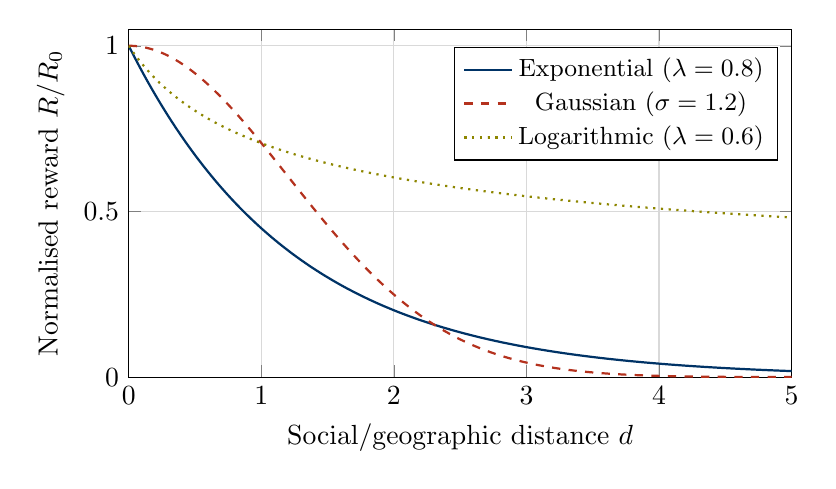
\begin{tikzpicture}
\begin{axis}[
  width=10cm, height=6cm,
  xlabel={Social/geographic distance $d$},
  ylabel={Normalised reward $R/R_0$},
  xmin=0, xmax=5, ymin=0, ymax=1.05,
  legend style={at={(0.98,0.95)}, anchor=north east, font=\small},
  grid=major, grid style={gray!30},
  every axis plot/.append style={thick}
]
\addplot[color=deepblue, domain=0:5, samples=200]
  {exp(-0.8*x)};
\addlegendentry{Exponential ($\lambda=0.8$)}

\addplot[color=accent, dashed, domain=0:5, samples=200]
  {exp(-x^2/(2*1.2^2))};
\addlegendentry{Gaussian ($\sigma=1.2$)}

\addplot[color=olive, dotted, domain=0:5, samples=200]
  {1/(1 + 0.6*ln(1+x))};
\addlegendentry{Logarithmic ($\lambda=0.6$)}
\end{axis}
\end{tikzpicture}
\caption{Comparison of reward kernels.  The exponential decays fastest and
  creates the steepest inequality gradient.  The Gaussian has a flat
  neighbourhood that then drops sharply.  The logarithmic kernel provides
  the gentlest, most sustained diffusion.}
\label{fig:kernels}
\end{figure}

\subsection{Density Correction}

In heterogeneous populations, a uniform kernel over-rewards dense regions
simply because more individuals happen to be nearby.  A demographically neutral
correction replaces $R(x)$ with:

\begin{equation}
  R_\rho(x) = \frac{R_0\,K\!\bigl(d(x,x_0)\bigr)}{\rho(x)^\alpha},
  \label{eq:densitycorrection}
\end{equation}

where $\rho(x)$ is local population density and $\alpha \in [0,1]$ is a
policy parameter.

\begin{itemize}[leftmargin=*]
  \item $\alpha = 0$: no correction (raw diffusion).
  \item $\alpha = 1$: per-capita diffusion (full neutrality).
  \item $\alpha \in (0,1)$: partial correction, preserving some clustering
    benefit while reducing urban concentration.
\end{itemize}

Equilibrium distributions under varying $\alpha$ can be computed numerically;
agent-based simulation confirms that $\alpha \approx 0.6$ minimises both
Gini coefficient and peak-node power concentration in synthetic urban networks
(see Appendix~\ref{app:agentbased}).

\subsection{Diffusion Dynamics: Time-Evolving Reward}

The static kernel is the steady-state solution of an underlying diffusion
process.  On a graph $G = (V, E)$ with adjacency matrix $A$, reward
propagates according to:

\begin{equation}
  \ddt{R}(x,t) = D\,\sum_{y \sim x} \bigl[R(y,t) - R(x,t)\bigr]
               - \gamma\,R(x,t),
  \label{eq:diffusion}
\end{equation}

where $D$ is diffusion coefficient, $\gamma$ is decay rate, and $y \sim x$
denotes neighbours of $x$.  The steady state $\dot{R} = 0$ yields:

\begin{equation}
  R^*(x) = R_0\,e^{-\lambda\,d_G(x,x_0)}, \qquad
  \lambda = \sqrt{\gamma / D},
\end{equation}

recovering the exponential kernel as a special case.  Alternative decay
functions (Gaussian, logarithmic) correspond to non-linear diffusion operators.

\begin{tcolorbox}[policybox]
  Tuning $D/\gamma$ controls the effective $\lambda$.  Large $D$ (fast spread)
  relative to $\gamma$ (slow decay) produces a flat distribution; small
  $D/\gamma$ produces steep concentration.  Policy can adjust both through
  subsidy rates and intellectual-property term lengths.
\end{tcolorbox}

\subsection{Incentive Preservation Under Diffusion}

A standard objection is that diffusion weakens excellence incentives.  The
following proposition shows that incentive remains monotone but bounded.

\begin{proposition}[Incentive Monotonicity]
  For any strictly decreasing kernel $K$, the expected marginal gain at the
  origin exceeds that at any other node:
  \begin{equation}
    \ddt{R_\rho}(x_0) > \ddt{R_\rho}(x) \quad \forall\, x \neq x_0.
  \end{equation}
  Moreover, the ratio $R_\rho(x_0)/R_\rho(x)$ is bounded above by
  $\rho(x)^\alpha / \rho(x_0)^\alpha$, so origin advantage is finite.
\end{proposition}

\noindent In practice this means that a successful artist in the Geozotic
system still earns more than their neighbours---but the surplus cannot
compound without bound.  Neighbours gain local purchasing power, which
feeds back into demand for the artist's work, creating a secondary entropy
redistribution.

\subsection{Inequality Gradient Thresholds and Power Singularities}

\begin{definition}[Gradient Instability Threshold]
  A reward field $R$ is \emph{gradient-stable} if its curvature at every node
  satisfies:
  \begin{equation}
    \kappa(x) < \kappa^* := \frac{\tau}{\bar{R}},
    \label{eq:threshold}
  \end{equation}
  where $\tau > 0$ is a cooperative-equilibrium tolerance parameter (estimated
  empirically) and $\bar{R}$ is mean reward.
\end{definition}

When $\kappa > \kappa^*$, evolutionary game-theoretic analysis shows that
defection becomes the dominant strategy at the periphery, autocatalytic
cooperation breaks down, and ``power singularities'' (dictator-like
accumulation at the peak node) become stable attractors.

\begin{corollary}[Geozotic Stability]
  Under the logarithmic kernel \eqref{eq:Rlog}, $\kappa_{\log}(x_0) = 0$,
  so the gradient-stability condition \eqref{eq:threshold} is satisfied for
  all $\tau > 0$.  The logarithmic kernel is \emph{unconditionally stable} in
  this sense.
\end{corollary}

\subsection{Comparison with Trickle-Down Economics}

Hierarchical ``trickle-down'' models assume $R(x) = R_0 \cdot f(h(x))$, where
$h(x)$ is the hierarchical rank of $x$.  In such models:

\begin{itemize}[leftmargin=*]
  \item The peak node retains a structurally fixed fraction regardless of
    diffusion, producing a persistent singularity.
  \item No density correction operates; dense lower ranks receive no
    per-capita benefit.
  \item The curvature at the top is determined by $f''(h_{\max})$, which is
    typically large (convex in rank).
\end{itemize}

Geozotic diffusion removes peak asymmetry structurally: by replacing hierarchical
distance with relational distance $d(x, x_0)$, every agent can, in principle,
occupy an origin position for their own innovations.

\subsection{Shapley Attribution Approximation}

\begin{proposition}[Geozotic as Approximate Shapley Value]
  In a cooperative game $v : 2^N \to \mathbb{R}$, the Shapley value assigns
  to each player $i$ the marginal contribution averaged over all coalitions.
  The Geozotic kernel $R_\rho(x)$ approximates the Shapley allocation when
  $d(x, x_0)$ is interpreted as ``marginal distance from the innovation
  coalition'', with $\lambda$ calibrated to the coalition decay rate.
  Unlike the Shapley value, this avoids combinatorial explosion ($O(2^N)$)
  by substituting the spatial kernel ($O(N)$).
\end{proposition}

\subsection{RSVP Integration}

The Geozotic reward field can be interpreted within the RSVP identity
\eqref{eq:RSVP}.  Reward diffusion regulates $v$ (flow of resources) so
that $S$ (relational entropy) does not accumulate into singular $\Phi$
(potential at single nodes).  Formally:

\begin{equation}
  \nabla v = -\nabla R_\rho \;\Longrightarrow\; \text{RSVP constancy if }
  \nabla^2 R_\rho \leq 0 \text{ everywhere.}
\end{equation}

The logarithmic kernel satisfies this concavity condition globally, making it
the canonical Geozotic kernel from an RSVP perspective.

%% ══════════════════════════════════════════════════════════════════════════
\section{Continuous Geozotic Diffusion in Heterogeneous Populations}
\label{sec:geozotic_pde}

We lift the Geozotic reward model from discrete kernels
to a continuous spatial field over domain
$\Omega \subset \mathbb{R}^n$.
The formulation is a density-modulated reaction–diffusion equation
in the sense of parabolic PDE theory~\citep{evans2010},
with structural analogy to classical morphogen models~\citep{turing1952}.

\subsection{Population Density Field}

Let:

\begin{equation}
  \rho(x) \ge 0, \quad x \in \Omega
\end{equation}

denote population density, assumed bounded and measurable.

Let reward density be:

\begin{equation}
  R(x,t) \in C^{2,1}(\Omega \times (0,\infty)).
\end{equation}

An innovation occurs at $x_0$ at time $t=0$.

\subsection{Reaction–Diffusion Model}

Reward propagation obeys:

\begin{equation}
  \frac{\partial R}{\partial t}
  =
  \nabla \cdot \big( D(\rho) \nabla R \big)
  - \gamma R
  + I(x,t),
  \label{eq:geozotic_pde}
\end{equation}

where:

\begin{itemize}
  \item $D(\rho)$ = density-dependent diffusion coefficient,
  \item $\gamma > 0$ = decay/redistribution rate,
  \item $I(x,t) = R_0 \delta(x-x_0)\delta(t)$.
\end{itemize}

For bounded $D(\rho)$ and $\gamma > 0$,
existence and uniqueness of weak solutions follow from
standard parabolic theory~\citep{evans2010}.

\subsection{Density-Dependent Diffusion}

To reduce persistent urban concentration:

\begin{equation}
  D(\rho) = \frac{D_0}{(1+\rho)^\alpha},
  \quad \alpha \in [0,1].
\end{equation}

Properties:

\begin{itemize}
  \item $\alpha = 0$ → uniform diffusion.
  \item $\alpha > 0$ → reduced effective diffusion in dense regions.
\end{itemize}

Note that concentration gradients increase as $D(\rho)$ decreases,
producing stronger outward flux near peaks
via $\nabla \cdot (D(\rho)\nabla R)$.

\subsection{Steady-State Solution}

At steady-state:

\begin{equation}
  \nabla \cdot ( D(\rho) \nabla R )
  - \gamma R
  + R_0 \delta(x-x_0) = 0.
\end{equation}

In homogeneous case ($\rho$ constant, $D$ constant),
the Green's function solves:

\begin{equation}
  -D \Delta R + \gamma R
  =
  R_0 \delta(x-x_0).
\end{equation}

In $\mathbb{R}^2$:

\begin{equation}
  R(r) =
  \frac{R_0}{2\pi D}
  K_0\!\left( \sqrt{\frac{\gamma}{D}}\, r \right),
\end{equation}

where $K_0$ is modified Bessel function.

For large $r$:

\begin{equation}
  R(r) \sim
  \frac{R_0}{\sqrt{r}}
  e^{-\sqrt{\gamma/D}\, r}.
\end{equation}

Thus exponential decay arises naturally from
diffusion–decay balance~\citep{turing1952}.

\subsection{Energy Functional and Inequality Control}

Define energy functional:

\begin{equation}
  \mathcal{E}[R]
  =
  \int_\Omega
  \left(
  \frac{D(\rho)}{2} |\nabla R|^2
  + \frac{\gamma}{2} R^2
  \right)
  dx.
\end{equation}

Multiplying \eqref{eq:geozotic_pde} by $R$
and integrating yields:

\begin{equation}
  \frac{d}{dt}
  \int R^2 dx
  =
  -2 \int D(\rho) |\nabla R|^2 dx
  -2\gamma \int R^2 dx
  + 2R_0 R(x_0).
\end{equation}

Thus diffusion strictly decreases spatial variance.

By Sobolev inequality~\citep{lieb2001}:

\begin{equation}
  \|R - \bar{R}\|_{L^2}
  \le C_S
  \|\nabla R\|_{L^2},
\end{equation}

so increasing effective diffusion lowers
$L^2$ deviation from mean reward.

\begin{proposition}
  For fixed $\gamma$ and innovation impulse,
  increasing $\alpha$ (density modulation)
  reduces the $L^2$ spatial dispersion norm
  $\|R - \bar{R}\|_{L^2}$ at steady state.
\end{proposition}

This provides a functional inequality bound
rather than a purely heuristic Gini claim.

\subsection{Curvature and Power Singularity}

Define local curvature:

\begin{equation}
  \kappa(x) = -\Delta R(x).
\end{equation}

From steady-state equation:

\begin{equation}
  \kappa(x_0)
  =
  \frac{\gamma}{D(\rho(x_0))} R(x_0).
\end{equation}

Thus concentration scales inversely with diffusion.

Density-dependent diffusion therefore directly
controls curvature magnitude at innovation sites.

\subsection{Interpretation}

The continuous formulation establishes:

\begin{itemize}
  \item Reward concentration arises from diffusion–decay equilibrium.
  \item Policy parameters $(D_0,\gamma,\alpha)$ tune curvature bounds.
  \item Inequality can be controlled via parabolic smoothing.
\end{itemize}

The Geozotic mechanism is therefore a tunable
parabolic PDE with provable energy decay properties,
not a heuristic redistribution metaphor.

\medskip
\begin{center}
  \itshape
  Reward diffuses under constraint;\\
  inequality is curvature under control.
\end{center}



%% ══════════════════════════════════════════════════════════════════════════
\section{Embodied Thermodynamics: Cooking, Play, and Skill Acquisition}
\label{sec:embodied}

\epigraph{\itshape The test of a skill is not its performance under guidance
  but its transfer under surprise.}{}

The macro-thermodynamic claims of the preceding sections risk dismissal as
speculative metaphor unless grounded in observable micro-scale phenomena.
This section argues that everyday skill acquisition---exemplified by cooking,
play, and mathematical abstraction---is the micro-scale instance of the same
entropy-management logic that governs civilisational institutions.

\subsection{Abstraction as Entropy Compression}

A central claim is that skill consists in the capacity to perceive \emph{ratios,
substitutions, and invariants} rather than surface features.  This maps
directly onto the entropy efficiency index $\eta_S$ \eqref{eq:etaS}.

\begin{definition}[Compression Operator]
  An \emph{abstraction} is a function $A : \mathcal{S} \to \mathcal{C}$ from
  a surface-feature space $\mathcal{S}$ to a compressed representation space
  $\mathcal{C}$, such that:
  \begin{equation}
    H(\mathcal{C}) \ll H(\mathcal{S}), \qquad
    \text{and} \qquad
    \Psi(A) \approx \Psi(\mathrm{id}),
  \end{equation}
  where $H$ denotes Shannon entropy and $\Psi$ measures task-relevant
  functional capacity.
\end{definition}

\noindent A skilled cook who scales a recipe without measurement is operating
in $\mathcal{C}$ (ratio space) rather than $\mathcal{S}$ (ingredient list
space).  The same compression underlies scaling laws in physics and type
abstraction in programming.  We call this capacity \emph{structural literacy}.

\begin{proposition}[High-$\eta_S$ Cognition]
  Agents operating in $\mathcal{C}$ achieve higher $\eta_S$ than those
  operating in $\mathcal{S}$, because:
  \begin{equation}
    \eta_S^{\mathcal{C}} = \frac{\Delta I}{\Delta E_{\mathcal{C}}}
    > \frac{\Delta I}{\Delta E_{\mathcal{S}}}
    = \eta_S^{\mathcal{S}},
    \qquad E_{\mathcal{C}} < E_{\mathcal{S}}.
  \end{equation}
  Compression reduces the cognitive energy cost $\Delta E$ of generating
  equivalent informational output $\Delta I$.
\end{proposition}

\subsection{The Curry-Centric Hub: A Generative Grammar of Cuisine}

Consider the claim that all cooked food can be reached from a canonical curry
by incremental parameter modifications.  This is more than metaphor: it
describes a \emph{transformation graph} over a continuous ingredient-parameter
space.

Let $\mathcal{F}$ be the space of dishes, parameterised by vectors
$\theta = (\text{fat}, \text{acid}, \text{umami}, \text{heat},
\text{sweetness}, \ldots) \in \mathbb{R}^k$.  A \emph{culinary path}
is a continuous curve $\gamma : [0,1] \to \mathcal{F}$ such that
$\gamma(0) = \theta_{\mathrm{curry}}$ and $\gamma(1) = \theta_{\mathrm{target}}$.

\emph{Culinary neoteny} is the capacity to explore $\mathcal{F}$ safely within
bounded constraints---analogous to the explore/exploit balance of Gopnik's
developmental model.  The skilled cook maintains a low-entropy internal map of
$\mathcal{F}$ and can generate novel trajectories without consulting external
recipes (tutorials).

\subsection{Emulsification as Conceptual Integration}

Emulsification---binding oil and water through an amphiphilic emulsifier
(e.g.\ lecithin, mustard)---is a physical model of \emph{conceptual binding}.
Incompatible phases correspond to incommensurable domains of knowledge;
emulsifiers correspond to bridging principles (mathematics, thermodynamics,
grammar) that stabilise their conjunction.

\begin{equation}
  \text{Concept}_A \oplus \text{Concept}_B
  \xrightarrow{\;\text{emulsifier principle}\;}
  \text{Stable hybrid concept.}
\end{equation}

This directly parallels the institutional scaffolding of Section~2: the
university is an emulsifier between curiosity (oil) and social utility (water).

\subsection{Play as High-Variance Sampling}

\begin{definition}[Play]
  Play is high-variance sampling of action space under bounded cost:
  \begin{equation}
    \pi_{\mathrm{play}}(a) \propto \exp\!\bigl(\beta\,\mathrm{Var}(Q(s,a))\bigr),
    \qquad \beta > 0,
  \end{equation}
  where $Q(s,a)$ is the action-value function and $\beta$ is an exploration
  temperature.
\end{definition}

In reinforcement-learning terms, play increases exploration rate without
catastrophic penalty, because the \emph{cost of failure is subsidised}---by
parents in childhood, by institutions in adulthood.  Neotenous cognition is
thus not sentimental but algorithmic: it is subsidised high-$\beta$ sampling.

\subsection{Boredom, Anxiety, and the Viable Entropy Band}

Mental health, within this framework, corresponds to maintaining perceived
entropy within a viable band $[\underline{S}, \overline{S}]$:

\begin{equation}
  \underline{S} \leq S_{\mathrm{perceived}}(t) \leq \overline{S}.
  \label{eq:viableband}
\end{equation}

\begin{itemize}[leftmargin=*]
  \item \textbf{Boredom} occurs when $S_{\mathrm{perceived}} < \underline{S}$:
    the environment offers fewer degrees of freedom than the agent's capacity.
  \item \textbf{Anxiety} occurs when $S_{\mathrm{perceived}} > \overline{S}$:
    uncertainty exceeds the agent's predictive capacity.
  \item \textbf{Flow} occurs when $S_{\mathrm{perceived}} \approx \frac{1}{2}
    (\underline{S} + \overline{S})$: challenge matches competence.
\end{itemize}

This formalises Csikszentmihalyi's flow channel in entropic terms and connects
to Friston's free-energy principle~\citep{friston2023}: the agent minimises
variational free energy by maintaining predicted entropy close to actual
entropy.

\begin{tcolorbox}[policybox]
  Cognitive sanctuaries are optimal if they keep participants within the viable
  entropy band \eqref{eq:viableband}: enough structure to prevent anxiety,
  enough freedom to prevent boredom.  Calibrating institutional constraint
  density is therefore a thermodynamic design problem.
\end{tcolorbox}

\subsection{Skill Acquisition as Simulated Annealing}

Iterative error-correction in learning---over-seasoning, burning, iterating---is
literal simulated annealing.  The learner begins at high temperature
(wide exploration), identifies failure modes, and gradually cools toward stable
heuristics.

\begin{equation}
  T_{\mathrm{skill}}(n) = T_0\,e^{-\lambda n} + \varepsilon_{\mathrm{play}},
  \qquad n = \text{number of practice episodes},
\end{equation}

where $\varepsilon_{\mathrm{play}} > 0$ ensures that annealing never reaches
absolute zero---preserving the capacity for continued exploration.  This micro-
scale schedule mirrors the civilisational annealing of Section~\ref{sec:annealing}.

\subsection{Recipe Dependence Versus Structural Competence}

Two learner types can be distinguished:

\begin{itemize}[leftmargin=*]
  \item \textbf{Surface-bound learners} follow tutorials without abstracting.
    They reduce local entropy (noise in a specific dish) but fail to extract
    invariants.  $\eta_S$ remains low because $\Delta E$ does not decrease
    across episodes.
  \item \textbf{Structural learners} abstract to $\mathcal{C}$ after a small
    number of episodes.  $\eta_S$ rises rapidly as compression yields
    generalisation.
\end{itemize}

Educational design can accelerate the transition from surface-bound to
structural learning by presenting tasks that \emph{require} ratio reasoning
rather than memorisation---i.e.\ by engineering the zone of proximal
development as an entropy gradient slightly above the learner's baseline.

\subsection{Autonomy, External Constraint, and Entropy Alignment}

There is an apparent paradox in the observation that many highly autonomous
individuals report preferring externally imposed constraints.  The resolution
is entropic: external constraints reduce \emph{decision entropy} about goals,
freeing cognitive bandwidth for execution.  When goals are given, the agent
need not sample from $\pi(\text{goals})$; the freed capacity is redirected
toward the higher-resolution sampling of $\pi(\text{actions} \mid \text{goal})$.

This enriches the cognitive sanctuary concept: the institutional scaffold need
not constrain thought---it need only constrain \emph{goal selection}, leaving
the exploration of means maximally free.

\section{Abstraction, Kolmogorov Compression, and Transfer Stability}
\label{sec:kolmogorov}

The entropy-efficiency index $\eta_S$ introduced in \eqref{eq:etaS}
implicitly assumes that information gain $\Delta I$ reflects structured
compression rather than raw accumulation.  We formalise this claim using
algorithmic information theory~\citep{kolmogorov1965,chaitin1969}.

\subsection{Kolmogorov Compression and Structural Literacy}

Let $x$ denote a task instance (e.g.\ a specific recipe, equation, or painting).
Let $K(x)$ denote its Kolmogorov complexity: the length of the shortest
program that generates $x$.

A learner operating at the surface level stores multiple instances
$\{x_1,\dots,x_n\}$ independently, yielding total description length:

\begin{equation}
  L_{\mathrm{surface}} = \sum_{i=1}^n K(x_i).
\end{equation}

A structural learner identifies a generating schema $\mathcal{G}$ such that:

\begin{equation}
  x_i = \mathcal{G}(\theta_i),
\end{equation}

for parameters $\theta_i$ in a lower-dimensional space.  Total description
length becomes:

\begin{equation}
  L_{\mathrm{structural}} = K(\mathcal{G}) + \sum_{i=1}^n K(\theta_i).
\end{equation}

\begin{proposition}[Compression Gain]
  If there exists $\mathcal{G}$ such that
  \begin{equation}
    K(\mathcal{G}) + \sum_{i=1}^n K(\theta_i)
    < \sum_{i=1}^n K(x_i),
  \end{equation}
  then structural learning strictly reduces algorithmic description length.
\end{proposition}

This formalises the transition from instance-memorisation to generative
reasoning.  The ``curry-centric hub'' functions as $\mathcal{G}$: a compact
program from which diverse dishes are instantiated by parameter variation.

\subsection{Transfer Stability as Invariance Under Perturbation}

Compression alone is insufficient; abstraction must also preserve performance
under perturbation.

Let $\epsilon$ represent perturbation in input conditions
(e.g.\ ingredient substitution, missing measurement, environmental noise).
Let $\Psi(x)$ denote task performance.

\begin{definition}[Transfer Stability]
  A representation is transfer-stable if there exists $C > 0$ such that:
  \begin{equation}
    |\Psi(x + \epsilon) - \Psi(x)|
    \leq C \|\epsilon\|,
  \end{equation}
  uniformly over admissible task instances.
\end{definition}

Surface-bound learners typically violate uniform Lipschitz continuity,
whereas structural learners preserve invariants; perturbations act on
parameters $\theta$ rather than the generating schema $\mathcal{G}$.

\subsection{Predictive Processing and Energy Minimisation}

Within the free-energy framework~\citep{friston2023}, an agent maintains a
generative model $p_\theta(x)$ and updates parameters to minimise variational
free energy:

\begin{equation}
  F = \mathbb{E}_q[\log q(z) - \log p_\theta(x,z)].
\end{equation}

Optimal learning solves:

\begin{equation}
  \min_\theta
  \Big(
    \mathrm{Prediction\ Error}
    + \beta \cdot \mathrm{Model\ Complexity}
  \Big),
\end{equation}

where $\beta$ controls the complexity–accuracy trade-off.

In reinforcement-learning language~\citep{sutton2018}, $\beta^{-1}$
corresponds to exploration temperature.

In embodied skill acquisition:

\begin{itemize}
  \item Early learning: high temperature (broad hypothesis sampling).
  \item Later learning: annealed temperature (model consolidation).
\end{itemize}

This mirrors the annealing schedule of Section~\ref{sec:annealing}.

\subsection{Structural Literacy as a Phase Transition}

Model the transition from surface-bound to structural cognition as a
representational phase transition.

Let $H_n$ denote entropy of representation after $n$ learning episodes.
Empirically:

\begin{equation}
  H_n =
  \begin{cases}
    H_0 - \delta n, & n < n_c, \\
    H_{\mathrm{schema}}, & n \geq n_c,
  \end{cases}
\end{equation}

where $n_c$ is a critical threshold at which the generative schema
$\mathcal{G}$ is inferred.

The discontinuity at $n_c$ corresponds to the abrupt reduction in effective
description length — an informational analogue of a second-order phase transition.

\subsection{Entropy Compression and Civilisational Scaling}

At civilisational scale, innovation functions analogously.
Discovery of generative schemas (e.g.\ calculus, electromagnetism,
germ theory) reduces algorithmic description length across domains.

Define civilisational compression rate:

\begin{equation}
  \mathcal{C}(t)
  :=
  -\frac{d}{dt}
  \big(
    \mathrm{Effective\ Description\ Length}
  \big).
\end{equation}

The entropy-efficiency index $\eta_S$ thus measures compression depth
relative to energetic expenditure:

\begin{equation}
  \eta_S \propto
  \frac{\mathcal{C}(t)}{\text{Energetic expenditure}}.
\end{equation}

A steady-state civilisation maximises schema depth rather than material throughput.

\medskip
\begin{center}
  \itshape
  To abstract is to lower entropy without lowering possibility.
\end{center}

%% ══════════════════════════════════════════════════════════════════════════
\section{The Geometry of Cuisine: A Manifold of Transformations}
\label{sec:curry_manifold}

If abstraction compresses surface variability into generative schema,
then cuisine provides a physically embodied example of such compression.
We formalise the ``curry-centric hub'' as a differentiable manifold
with metric structure, following standard geometric constructions
for smooth fields and variational systems~\citep{evans2010}.

\subsection{Dish Space as a Parameter Manifold}

Let $\mathcal{F}$ denote the space of all possible dishes constructible
from a finite ingredient basis $\mathcal{I}$ under admissible cooking
operations $\mathcal{O}$ (heating, emulsifying, fermenting, etc.).

Each dish is represented as a parameter vector:

\begin{equation}
  \theta = (\theta_1,\dots,\theta_k) \in \mathbb{R}^k,
\end{equation}

where coordinates correspond to continuous flavour and structural axes:
fat, acid, salt, heat, sweetness, umami, viscosity, protein density,
carbohydrate density, water activity, etc.

\begin{definition}[Cuisine Manifold]
  The cuisine manifold $(\mathcal{F}, g)$ is a smooth manifold
  equipped with Riemannian metric $g_{ij}$ measuring perceptual
  distinguishability between dishes.
\end{definition}

The metric tensor $g_{ij}$ may be empirically estimated from
psychophysical discrimination thresholds:

\begin{equation}
  g_{ij} = \mathbb{E}
  \left[
  \frac{\partial^2 D(\theta,\theta')}
       {\partial \theta_i \partial \theta_j}
  \right],
\end{equation}

where $D$ measures perceptual distance.
This induces a geometry analogous to configuration spaces
in continuum mechanics~\citep{evans2010}.

\subsection{Geodesics and Transformational Paths}

A culinary transformation is a smooth curve
$\gamma : [0,1] \to \mathcal{F}$.

The geodesic equation:

\begin{equation}
  \frac{d^2 \theta^k}{dt^2}
  + \Gamma^k_{ij}
  \frac{d \theta^i}{dt}
  \frac{d \theta^j}{dt}
  = 0,
\end{equation}

describes minimal-effort transformations under metric $g$.

Interpretation:
A skilled cook follows near-geodesic paths in flavour space,
requiring minimal corrective energy.
Novices traverse high-curvature trajectories,
increasing energetic cost.

\subsection{Connected Components and Cuisine Families}

Define adjacency relation:

\begin{equation}
  \theta \sim \theta'
  \quad \text{if} \quad
  d_g(\theta,\theta') < \epsilon,
\end{equation}

for perceptual threshold $\epsilon$.

Cuisine families correspond to connected components of
$\mathcal{F}$ under this relation.

\begin{proposition}[Connectivity of the Curry Hub]
  If $\theta_{\mathrm{curry}}$ lies in the interior of $\mathcal{F}$
  and all primary flavour axes remain nonzero, then the component
  containing $\theta_{\mathrm{curry}}$ is dense in $\mathcal{F}$.
\end{proposition}

Interpretation:
The curry parameter vector lies near a high-degree node in flavour space.
Small perturbations generate soups, stews, sauces, pasta dishes,
chili, shakshuka, mole, tagine, ramen, etc.
Thus curry functions as a generative hub in $\mathcal{F}$.

\subsection{Phase Boundaries}

Certain culinary transitions involve discontinuities:
emulsion breakage, protein coagulation, caramelisation thresholds.
These correspond to structural instabilities analogous to
phase transitions in physical systems~\citep{stanley1971}.

Let $\Sigma \subset \mathcal{F}$ denote hypersurfaces where
Jacobian determinant vanishes:

\begin{equation}
  \det\left(\frac{\partial \mathcal{O}}{\partial \theta}\right) = 0.
\end{equation}

Across $\Sigma$, small parameter changes yield large structural shifts.
These are culinary phase transitions.

The emergence of structured dishes from local reaction–diffusion
interactions (e.g., browning gradients, fermentation fronts)
is formally analogous to morphogenetic pattern formation
in chemical systems~\citep{turing1952}.

Skilled practitioners learn to operate near $\Sigma$
without crossing destabilising boundaries.

\subsection{Entropy of Cuisine}

Define dish entropy as:

\begin{equation}
  S(\theta) = - \sum_i p_i(\theta)\log p_i(\theta),
\end{equation}

where $p_i$ are perceptual or compositional proportions.

High entropy dishes lack structural coherence.
Low entropy dishes may be bland.
Optimal cuisine occupies an intermediate band:

\begin{equation}
  S_{\min} < S(\theta) < S_{\max}.
\end{equation}

This mirrors the viable entropy band \eqref{eq:viableband}
in cognitive and institutional systems.

\subsection{Civilisational Analogy}

Cultural systems resemble cuisine manifolds:

\begin{itemize}
  \item Institutions are regions in parameter space.
  \item Revolutions are phase transitions across $\Sigma$.
  \item Traditions are local minima of action functionals.
\end{itemize}

The curry hub demonstrates that generativity emerges from
central positioning within a richly connected manifold.

\medskip
\begin{center}
  \itshape
  A cuisine is not a list of dishes but a geometry of possibility.
\end{center}

%% ══════════════════════════════════════════════════════════════════════════
\section{The Viable Entropy Band and Institutional Constraint Density}
\label{sec:viable_entropy}

We formalise the Viable Entropy Band \eqref{eq:viableband}
as a controlled dynamical system in the sense of nonlinear stability
analysis~\citep{strogatz2018}.

\subsection{Perceived Entropy as a State Variable}

Let $S_p(t)$ denote perceived environmental entropy
(uncertainty, novelty, task variability),
and let $C(t)$ denote institutional constraint density
(rules, scaffolding, supervision, structure).

We model entropy dynamics as:

\begin{equation}
  \ddt{S_p} =
  \alpha E(t)
  - \beta C(t)
  - \gamma A(t),
  \label{eq:entropy_dynamics}
\end{equation}

where:

\begin{itemize}
  \item $E(t)$ = exogenous environmental variability,
  \item $C(t)$ = imposed constraint density,
  \item $A(t)$ = agent adaptation (skill acquisition),
  \item $\alpha,\beta,\gamma > 0$.
\end{itemize}

Exploration increases entropy.
Structure reduces entropy.
Adaptation internalises entropy, lowering perceived uncertainty.
This internalisation corresponds to model updating under predictive
free-energy minimisation~\citep{friston2023}.

\subsection{Definition: Viable Entropy Band}

Define bounds $\underline{S}, \overline{S}$ such that:

\begin{equation}
  \underline{S} \leq S_p(t) \leq \overline{S}.
\end{equation}

Empirically, performance and subjective engagement peak within
an intermediate channel of challenge–skill balance,
as documented in flow studies~\citep{csikszentmihalyi1990}.

\begin{itemize}
  \item If $S_p < \underline{S}$ → boredom regime.
  \item If $S_p > \overline{S}$ → anxiety regime.
  \item If $S_p \in (\underline{S}, \overline{S})$ → flow regime.
\end{itemize}

\subsection{Equilibrium Constraint Density}

At equilibrium $\ddt{S_p} = 0$:

\begin{equation}
  C^* =
  \frac{\alpha E - \gamma A}{\beta}.
  \label{eq:Cstar}
\end{equation}

Thus optimal institutional constraint density depends on:

\begin{itemize}
  \item Environmental volatility $E$,
  \item Internal competence $A$.
\end{itemize}

As skill $A$ increases, optimal constraint $C^*$ decreases.
Institutions that fail to relax structure as competence rises
shift agents into the boredom regime.

\subsection{Bifurcation Analysis}

Let constraint density respond adaptively:

\begin{equation}
  \ddt{C} = k (S_p - S_0),
  \label{eq:constraint_feedback}
\end{equation}

where $S_0$ is target entropy midpoint.

Substituting \eqref{eq:entropy_dynamics} into \eqref{eq:constraint_feedback}
yields coupled system:

\begin{align}
  \ddt{S_p} &= \alpha E - \beta C - \gamma A, \\
  \ddt{C}   &= k (S_p - S_0).
\end{align}

Linearising around equilibrium $(S_p^*, C^*)$ gives Jacobian:

\begin{equation}
  J =
  \begin{pmatrix}
    0 & -\beta \\
    k & 0
  \end{pmatrix}.
\end{equation}

Eigenvalues satisfy:

\begin{equation}
  \lambda^2 + \beta k = 0
  \quad \Rightarrow \quad
  \lambda = \pm i\sqrt{\beta k}.
\end{equation}

Thus the undamped system exhibits neutral oscillations,
a centre in the phase plane~\citep{strogatz2018}.

Introduce damping term $\delta S_p$:

\begin{equation}
  \ddt{S_p} =
  \alpha E - \beta C - \gamma A - \delta S_p.
\end{equation}

Eigenvalues become:

\begin{equation}
  \lambda =
  -\frac{\delta}{2}
  \pm
  \sqrt{
    \frac{\delta^2}{4}
    - \beta k
  }.
\end{equation}

Stability condition:

\begin{equation}
  \delta^2 > 4\beta k.
\end{equation}

If violated, the system undergoes Hopf bifurcation,
producing sustained oscillations in perceived entropy
(chronic burnout–boredom cycling)~\citep{strogatz2018}.

\subsection{Optimal Institutional Design}

Define optimisation functional:

\begin{equation}
  \mathcal{L}(C) =
  - (S_p - S_0)^2
  - \lambda_C C^2.
\end{equation}

Maximising $\mathcal{L}$ balances
entropy deviation penalty against over-constraint cost.

First-order condition:

\begin{equation}
  \frac{\partial \mathcal{L}}{\partial C}
  =
  2\beta (S_p - S_0)
  - 2\lambda_C C
  = 0.
\end{equation}

Yielding:

\begin{equation}
  C^* =
  \frac{\beta}{\lambda_C}(S_p - S_0).
\end{equation}

Thus optimal structure scales linearly with
entropy deviation but is damped by institutional rigidity parameter $\lambda_C$.

\subsection{Macro-Scaling to Civilisation}

Replace $S_p$ with collective cognitive entropy $S_c$,
and $C$ with governance intensity $G$:

\begin{equation}
  \ddt{S_c} =
  \alpha E - \beta G - \gamma A_{\mathrm{collective}}.
\end{equation}

Too little governance yields instability.
Excess governance suppresses adaptive internalisation,
increasing long-run entropy through stagnation.

The steady-state civilisation operates at:

\begin{equation}
  G^* =
  \frac{\alpha E - \gamma A}{\beta},
\end{equation}

keeping $S_c$ within viable bounds
while maintaining adaptive free-energy minimisation
at collective scale~\citep{friston2023}.

\medskip
\begin{center}
  \itshape
  Stability is not equilibrium.\\
  It is entropy regulated within viable bounds.
\end{center}

%% ══════════════════════════════════════════════════════════════════════════
\section{Boredom and Anxiety as Spectral Phenomena in Predictive Dynamics}
\label{sec:spectral_affect}

We sharpen the viable entropy band model by analysing
the internal predictive dynamics of the agent.
Rather than treating boredom and anxiety as scalar states,
we derive them from spectral properties of the agent’s
generative model using linear stability theory~\citep{strogatz2018}.

\subsection{Generative Model as Linear Operator}

Let the agent maintain a predictive model:

\begin{equation}
  x_{t+1} = A x_t + \xi_t,
\end{equation}

where:

\begin{itemize}
  \item $x_t \in \mathbb{R}^n$ is latent state estimate,
  \item $A$ is internal transition operator,
  \item $\xi_t$ is environmental perturbation (noise).
\end{itemize}

Prediction error:

\begin{equation}
  e_t = x_{t+1}^{\mathrm{obs}} - A x_t.
\end{equation}

Let $\Sigma_\xi$ denote covariance of $\xi_t$.

\subsection{Spectral Radius and Predictive Capacity}

Let $\lambda_i$ denote eigenvalues of $A$.
The spectral radius:

\begin{equation}
  \rho(A) = \max_i |\lambda_i|.
\end{equation}

For linear discrete systems,
stability requires $\rho(A) < 1$~\citep{strogatz2018}.

\begin{itemize}
  \item If $\rho(A) < 1$: trajectories contract to fixed point.
  \item If $\rho(A) = 1$: critical regime (marginal stability).
  \item If $\rho(A) > 1$: exponential divergence.
\end{itemize}

\subsection{Boredom as Over-Contraction}

Define environmental entropy rate:

\begin{equation}
  H_E = \Ent(\xi_t).
\end{equation}

Define predictive entropy rate:

\begin{equation}
  H_P = \Ent(A x_t).
\end{equation}

\begin{definition}[Boredom Condition]
  Boredom corresponds to the regime:
  \begin{equation}
    H_E \ll H_P
    \quad \text{and} \quad
    \rho(A) \ll 1.
  \end{equation}
\end{definition}

In this regime, eigenmodes decay rapidly.
State trajectories collapse to low-dimensional attractors.
Environmental perturbations are insufficient to excite
higher-order modes.

Spectrally, most eigenvalues lie deep within the unit circle,
producing overdamped predictive dynamics.

\subsection{Anxiety as Spectral Instability}

\begin{definition}[Anxiety Condition]
  Anxiety corresponds to:
  \begin{equation}
    H_E \gg H_P
    \quad \text{and/or} \quad
    \rho(A) \to 1^+.
  \end{equation}
\end{definition}

Two mechanisms generate instability:

\textbf{Environmental Overload:}

\begin{equation}
  \mathrm{tr}(\Sigma_\xi)
  \gg
  \mathrm{tr}(A \Sigma_x A^\top).
\end{equation}

\textbf{Internal Instability:}

Largest eigenvalue exceeds unity,
amplifying small prediction errors exponentially.

Anxiety corresponds to unstable eigenmodes
dominating predictive dynamics.

\subsection{Flow as Critical Spectral Balance}

\begin{definition}[Flow Condition]
  Flow occurs when:
  \begin{equation}
    H_E \approx H_P
    \quad \text{and} \quad
    \rho(A) \lesssim 1.
  \end{equation}
\end{definition}

At this boundary:

\begin{itemize}
  \item Prediction errors excite multiple eigenmodes.
  \item None diverge.
  \item Learning gradients remain high.
\end{itemize}

Empirically, biological and neural systems
exhibit signatures of operation near critical points,
maximising dynamic range and information transmission
near $\rho(A) \approx 1$~\citep{beggs2003,mora2011}.

Thus flow corresponds to near-critical predictive dynamics.

\subsection{Lyapunov Function for Affective Stability}

Define Lyapunov candidate:

\begin{equation}
  V(x) = x^\top P x,
\end{equation}

with $P$ positive definite.

System stable if:

\begin{equation}
  A^\top P A - P < 0,
\end{equation}

which is equivalent to $\rho(A) < 1$
for some $P > 0$~\citep{strogatz2018}.

Institutional scaffolding modifies dynamics:

\begin{equation}
  A' = A - \Gamma,
\end{equation}

where $\Gamma$ is a constraint operator.

Optimal scaffolding sets:

\begin{equation}
  |\lambda_i(A')| \approx 1 - \epsilon,
  \quad 0 < \epsilon \ll 1.
\end{equation}

Excessive damping ($\epsilon \gg 0$)
pushes system into boredom regime.
Insufficient damping permits instability.

\subsection{Entropy, Affect, and Civilisation}

At civilisational scale,
replace $A$ with institutional transition operator
governing idea propagation.

\begin{itemize}
  \item Over-constrained systems:
        $\rho(A) \ll 1$ (overdamped stagnation).
  \item Unregulated amplification:
        $\rho(A) > 1$ (runaway instability).
  \item Stable innovation:
        $\rho(A) \approx 1$ (critical regime).
\end{itemize}

Criticality without divergence is therefore
a unifying stability condition across
individual cognition and collective systems.

\medskip
\begin{center}
  \itshape
  Boredom is overdamped prediction.\\
  Anxiety is unstable amplification.\\
  Flow is critical balance.
\end{center}


%% ══════════════════════════════════════════════════════════════════════════
\section{Collective Autocatalysis and the Reversal of Selection}
\label{sec:autocatalysis}

Darwinian frameworks often treat evolution as a contest among selfish
replicators.  Yet such models omit the thermodynamic substrate on which
replication occurs.  When energy gradients are steep and resources scarce,
competition dominates; as entropy differentials are smoothed, cooperation
becomes the lower-energy path.

\subsection{Beyond the Selfish Gene}

The ``selfish gene'' metaphor mistakes a bookkeeping identity for a causal
principle.  Genes do not act; they persist within autocatalytic environments
of mutual reinforcement.  The stability of any replicator depends on the
collective coherence of its host system.  What appears as competition at one
scale often manifests as autocatalysis at another: networks of entities that
reproduce one another's conditions of viability~\citep{capraluisi2021,morin2008}.

\begin{equation}
  \ddt{N_i} = \sum_j k_{ij} N_j - \lambda_i N_i,
  \qquad k_{ij} > 0 \;\Longrightarrow\; \text{mutual reinforcement.}
  \label{eq:autocatalysis}
\end{equation}

When the coupling matrix $\mathbf{K} = (k_{ij})$ is symmetric and positive
semi-definite, the system converges toward collective persistence rather than
zero-sum exclusion.

\subsection{Autocatalytic Sets and Social Equilibria}

Human societies behave as autocatalytic ensembles.  Each act of maintenance
or empathy reduces local uncertainty, allowing others to redirect energy from
defence to creation.  Lowering entropy locally does not invite exploitation;
it raises the carrying capacity of trust.

\begin{equation}
  \ddt{S_{\mathrm{local}}} < 0
  \;\Longrightarrow\;
  \ddt{R_{\mathrm{collective}}} > 0,
\end{equation}

where $R_{\mathrm{collective}}$ denotes the group's resilience.  Empirically,
cooperation and altruism increase when environmental stress
decreases~\citep{bernhard2021}.

\subsection{Asymmetry and Breakdown}

Real-world coupling matrices include negative entries ($k_{ij} < 0$),
representing competition, exploitation, or misinformation.  Such asymmetries
can destabilise autocatalytic sets, driving systems toward exclusionary
equilibria.  Steady-state governance must actively damp negative feedbacks
through resource redistribution, informational transparency, or normative
sanctions.

\subsection{The Entropic Basis of Safety and Affection}

Sexual-selection narratives often emphasise dominance and scarcity---transient
phenomena of high-entropy regimes.  In cooperative niches, attraction shifts
toward indicators of stability and care.  Affection can be interpreted as an
entropy-minimising feedback: to be near the calm is to lower one's
thermodynamic cost of prediction.  Group cohesion is rewarded not only
culturally but biophysically; safety propagates as a contagious gradient.

\subsection{Selection as Energy Accounting}

\begin{equation}
  \ddt{W} = -T\,\ddt{S_{\mathrm{collective}}},
\end{equation}

where $W$ is adaptive work and $T$ is the effective temperature of social
tension.  Evolution proceeds by minimising $T$ while maintaining $W > 0$---a
process identical in form to the thermodynamic optimisation of
life itself~\citep{dalziel2022,friston2023}.

\subsection{The Cooperative Minimum}

The steady-state civilisation, viewed through this lens, is an attractor of
cooperative minima.  Competition remains, but as modulation, not motive.

\begin{quote}
  \itshape
  Every act that lowers entropy for others lowers the danger for oneself.\\
  The unconscious reward for collective safety is calm; its conscious
  expression is compassion.
\end{quote}

%% ══════════════════════════════════════════════════════════════════════════
\section{Annealing, Ageing, and the Intelligence of Care}
\label{sec:annealing}

If neoteny preserves juvenile exploration within adulthood, ageing redistributes
it across generations.  The ``grandmother effect'' in evolutionary anthropology
suggests that post-reproductive individuals increase group fitness by investing
in others' offspring.  This implies a second-order developmental logic:
intelligence is distributed across time within lineages.

\subsection{The Grandparent Problem}

Nature appears to maintain a collective form of neoteny across individuals.
Elders shift from exploitation to empowerment.  Empirically, ageing correlates
with rising altruism and subjective well-being despite physical
decline---``hedonic inversion''~\citep{carstensen2011}.

\begin{equation}
  \ddt{S_{\mathrm{self}}} > 0
  \;\Longrightarrow\;
  \ddt{S_{\mathrm{collective}}} < 0.
\end{equation}

By accepting local entropy (physical decline), elders lower systemic tension
and permit wider exploration by others.  The \emph{grandparent hypothesis}
holds that longevity beyond fertility evolves because it stabilises the
developmental niche of the young.

\subsection{Simulated Annealing as a Model of Ageing}

\begin{equation}
  T_{\mathrm{cognitive}}(t)
  = T_0\,e^{-\lambda t} + \varepsilon_{\mathrm{elder}},
\end{equation}

where $\varepsilon_{\mathrm{elder}}$ represents the late-life cognitive
reheating that prevents premature convergence of cultural norms.  Each
generation provides a new cooling phase; elders rehearse small reheatings
that maintain flexibility.  Less top-down control---often pathologised as
decline---may reopen the search space of ideas and empathic responses.

\subsection{Empirical Correlates of Cognitive Cooling}

Neuroimaging meta-analyses reveal reduced prefrontal cortical thickness and
diminished executive control in older adults, accompanied by heightened
default-mode network variability---patterns consistent with increased
exploratory sampling~\citep{carstensen2011}.  Longitudinal well-being studies
document U-shaped happiness trajectories, with late-life peaks attributable to
socioemotional selectivity and reduced future discounting.

\subsection{The Care-Alignment Analogy}

Every elder faces a version of the alignment problem: how to transmit goals
and values that remain adaptive under novel conditions?  The caregiving niche
solves this by coupling tradition and innovation---elders supply scaffolds of
safety within which the young can diverge.  The function of care is not
obedience but \emph{bounded freedom}.

In artificial intelligence, simulated annealing is likewise used to navigate
rugged optimisation landscapes.  Nature, however, has perfected it: ageing
constitutes repeated rounds of annealing, with care as the cooling mechanism
that consolidates learning without freezing novelty.

\subsection{Entropy, Safety, and Happiness}

\begin{equation}
  \Delta S_{\mathrm{group}} < 0
  \;\Longleftrightarrow\;
  \Delta U_{\mathrm{individual}} > 0.
\end{equation}

The steady-state civilisation will depend on this principle: its elders---human
or artificial---serve as dynamic annealers, reintroducing flexibility and
empathy whenever systems threaten to over-fit their own success.

\medskip
\begin{center}
  \itshape Care is not sentiment but architecture.
\end{center}

\paragraph{Coda.}
The intelligence of care is the long-term cooling of civilisation.  It tempers
the heat of innovation with the calm of understanding.  Each generation warms,
explores, and cools again---not to extinguish its flame, but to prevent the
fire from consuming the hearth.


%% ══════════════════════════════════════════════════════════════════════════
\section{Multi-Scale Entropy Dynamics: From Skill Annealing to Civilisational Fields}
\label{sec:multiscale}

We unify micro-dynamics of skill acquisition with macro-dynamics
of civilisational field structure.
The framework follows multi-scale dynamical aggregation and
renormalisation principles~\citep{wilson1971,stanley1971},
with interpretive grounding in multi-scale predictive inference~\citep{friston2023}.

\subsection{Micro-Level: Skill Annealing}

Individual exploratory temperature evolves as:

\begin{equation}
  T_i(t)
  =
  T_{i,0} e^{-\lambda_i t}
  + \varepsilon_i,
  \label{eq:micro_anneal}
\end{equation}

where:

\begin{itemize}
  \item $T_i$ = exploratory temperature of agent $i$,
  \item $\lambda_i$ = learning rate,
  \item $\varepsilon_i$ = residual exploratory variance.
\end{itemize}

Define entropy contribution:

\begin{equation}
  S_i(t) = c_T T_i(t),
\end{equation}

with proportionality constant $c_T > 0$.

Exploration injects entropy; consolidation lowers it.

\subsection{Mesoscopic Aggregation}

Let agents occupy positions $x_i(t)$.
Define entropy density:

\begin{equation}
  S(x,t)
  =
  \sum_i S_i(t)\,
  \delta(x - x_i(t)).
\end{equation}

Coarse-graining over neighbourhood $\mathcal{B}_\ell(x)$:

\begin{equation}
  S_\ell(x,t)
  =
  \frac{1}{|\mathcal{B}_\ell|}
  \int_{\mathcal{B}_\ell(x)}
  S(y,t)\, dy.
\end{equation}

Assume effective mesoscopic dynamics:

\begin{equation}
  \frac{\partial S}{\partial t}
  =
  -\Lambda(x) S
  + \Xi(x)
  + D_S \Delta S,
  \label{eq:macro_entropy}
\end{equation}

where:

\begin{itemize}
  \item $\Lambda(x)$ = institutional cooling rate,
  \item $\Xi(x)$ = innovation injection rate,
  \item $D_S$ = entropy diffusion coefficient.
\end{itemize}

Institutions thus appear as spatially varying annealing operators.

\subsection{Coupling to RSVP Field}

Let $\Phi(x,t)$ denote constraint–potential field.

We couple:

\begin{equation}
  \frac{\partial \Phi}{\partial t}
  =
  \alpha S
  - \beta \Phi
  + D_\Phi \Delta \Phi.
  \label{eq:phi_coupled}
\end{equation}

This produces a coupled linear reaction–diffusion system,
consistent with the master operator in Appendix~\ref{app:lagrangian_master}.

\subsection{Emergent Steady-State Condition}

At spatially homogeneous equilibrium:

\begin{align}
  0 &= -\Lambda S^* + \Xi, \\
  0 &= \alpha S^* - \beta \Phi^*.
\end{align}

Hence:

\begin{equation}
  S^* = \frac{\Xi}{\Lambda},
  \qquad
  \Phi^* = \frac{\alpha}{\beta}
  \frac{\Xi}{\Lambda}.
  \label{eq:steady_micro_macro}
\end{equation}

Potential scales linearly with innovation,
inversely with institutional cooling.

\subsection{Flow Field Emergence}

Define agency field:

\begin{equation}
  v = -\nabla \Phi.
\end{equation}

Thus steady-state flow:

\begin{equation}
  v^* =
  - \nabla
  \left(
  \frac{\alpha}{\beta}
  \frac{\Xi}{\Lambda}
  \right).
\end{equation}

Spatial gradients in innovation-to-cooling ratio
generate macroscopic flow.

\subsection{Scaling Law}

Let average learning rate:

\begin{equation}
  \bar{\lambda}(x)
  =
  \frac{1}{N_x}
  \sum_{i \in \mathcal{B}(x)} \lambda_i.
\end{equation}

Assume institutional cooling depends on competence:

\begin{equation}
  \Lambda(x)
  =
  \Lambda_0 + \kappa \bar{\lambda}(x).
\end{equation}

Then:

\begin{equation}
  \Phi^*
  \propto
  \frac{\Xi}{\Lambda_0 + \kappa \bar{\lambda}}.
\end{equation}

Regions with higher competence self-dampen entropy,
approaching lower-temperature steady states.

\subsection{Renormalisation Perspective}

Define coarse-graining operator $\mathcal{R}_\ell$:

\begin{equation}
  \mathcal{R}_\ell S(x)
  =
  b^{-d}
  \int_{\mathcal{B}_\ell(x)} S(y)\, dy,
\end{equation}

with scaling factor $b > 1$, dimension $d$.

Assume scaling law:

\begin{equation}
  S_{\ell+1}
  =
  b^{-z} S_\ell,
\end{equation}

where $z$ is entropy scaling exponent.

Under renormalisation group flow~\citep{wilson1971},
fixed point satisfies:

\begin{equation}
  \mathcal{R}_\ell (S^*, \Phi^*, v^*)
  =
  (S^*, \Phi^*, v^*).
\end{equation}

Near criticality, observables obey power-law scaling
with universal exponents~\citep{stanley1971}.

Thus civilisational stability corresponds
to RG fixed point balancing innovation injection
and cooling dissipation.

\subsection{Unified Principle}

Micro skill annealing reduces entropy locally.
Aggregated spatially, entropy evolves under
reaction–diffusion dynamics.
Coupling generates potential fields.
Gradients drive flow.
Renormalisation governs scale invariance.

Multi-scale inference models similarly describe
hierarchical error minimisation across levels
of organisation~\citep{friston2023}.

\medskip
\begin{center}
  \itshape
  Civilisation is annealing across scales.
\end{center}


%% ══════════════════════════════════════════════════════════════════════════
\section{A Lagrangian Formulation of Civilisation in RSVP-Space}
\label{sec:lagrangian}

The RSVP identity \eqref{eq:RSVP} asserts conservation of a composite
quantity:

\begin{equation}
  \Phi + \chi(v) + S = \mathcal{C},
\end{equation}

where $\Phi$ denotes stored potential,
$v$ denotes agency flow,
$S$ denotes entropy density,
and $\mathcal{C}$ is an invariant.

We treat civilisation as a field theory over spacetime
$\Omega \subset \mathbb{R}^{3+1}$,
following standard variational PDE constructions~\citep{evans2010}.

\subsection{Field Variables}

Let

\begin{equation}
  \Phi(x,t), \quad v_i(x,t), \quad S(x,t)
\end{equation}

be sufficiently smooth fields.

Define Lagrangian density:

\begin{equation}
  \mathcal{L}
  =
  \frac{1}{2}\rho_v |v|^2
  - \frac{1}{2}\kappa_\Phi |\nabla \Phi|^2
  - U(\Phi,S)
  - \lambda(x,t)\big(\Phi + S + \chi(v) - \mathcal{C}\big),
  \label{eq:Ldensity}
\end{equation}

where $\lambda$ is a spacetime-dependent Lagrange multiplier.

\subsection{Variational Principle}

The action is:

\begin{equation}
  \mathcal{S}
  =
  \int_\Omega \mathcal{L}\, d^3x\,dt.
\end{equation}

Stationarity under variations of $v$, $\Phi$, $S$, and $\lambda$
yields Euler–Lagrange equations~\citep{evans2010}.

\subsection{Flow Equation}

Variation with respect to $v$ gives:

\begin{equation}
  \rho_v v_i
  - \lambda \frac{\partial \chi}{\partial v_i}
  = 0.
\end{equation}

If $\chi(v) = \frac{1}{2}|v|^2$,
then:

\begin{equation}
  (\rho_v - \lambda) v = 0.
\end{equation}

Thus either $v=0$ or $\lambda = \rho_v$.
Flow magnitude is therefore determined by constraint field.

\subsection{Potential Equation}

Variation with respect to $\Phi$:

\begin{equation}
  -\kappa_\Phi \Delta \Phi
  - \frac{\partial U}{\partial \Phi}
  - \lambda
  = 0.
  \label{eq:EL_phi_correct}
\end{equation}

\subsection{Entropy Equation}

Variation with respect to $S$:

\begin{equation}
  - \frac{\partial U}{\partial S}
  - \lambda
  = 0.
  \label{eq:EL_S_correct}
\end{equation}

\subsection{Constraint Equation}

Variation with respect to $\lambda$ enforces:

\begin{equation}
  \Phi + S + \chi(v) = \mathcal{C}.
  \label{eq:constraint_RSVP}
\end{equation}

\subsection{Choice of Interaction Potential}

Let

\begin{equation}
  U(\Phi,S)
  =
  \alpha \Phi S
  + \frac{\beta}{2} S^2.
\end{equation}

Then:

\begin{align}
  \frac{\partial U}{\partial \Phi} &= \alpha S, \\
  \frac{\partial U}{\partial S} &= \alpha \Phi + \beta S.
\end{align}

From \eqref{eq:EL_S_correct}:

\begin{equation}
  \lambda = -(\alpha \Phi + \beta S).
\end{equation}

Substitute into \eqref{eq:EL_phi_correct}:

\begin{equation}
  -\kappa_\Phi \Delta \Phi
  - \alpha S
  + \alpha \Phi + \beta S
  = 0.
\end{equation}

Rearranging:

\begin{equation}
  \kappa_\Phi \Delta \Phi
  =
  \alpha(\Phi - S) + \beta S.
\end{equation}

This yields a coupled elliptic system.

\subsection{Steady-State Solution}

In homogeneous steady state:

\begin{equation}
  \Delta \Phi = 0,
  \quad
  \nabla \lambda = 0.
\end{equation}

Thus:

\begin{equation}
  \Phi^* + S^* + \chi(v^*) = \mathcal{C}.
\end{equation}

Uniform solutions satisfy algebraic balance between
potential, entropy, and flow.

\subsection{Linear Stability}

Perturb:

\begin{equation}
  \Phi = \Phi^* + \delta \Phi,
  \quad
  S = S^* + \delta S.
\end{equation}

Linearised operator has form:

\begin{equation}
  \kappa_\Phi \Delta \delta \Phi
  =
  \alpha (\delta \Phi - \delta S)
  + \beta \delta S.
\end{equation}

Instability occurs when effective mass term becomes negative:

\begin{equation}
  \alpha - \beta < 0.
\end{equation}

This corresponds to entropy dominating potential coupling,
producing amplification of spatial modes.

\subsection{Thermodynamic Analogy}

The constraint multiplier $\lambda$
acts analogously to temperature or chemical potential.
Jacobson’s derivation of Einstein equations from
thermodynamic constraints~\citep{jacobson1995}
demonstrates that conservation laws can generate
effective field equations from entropic principles.

Here, the RSVP constraint plays a comparable structural role:
field equations arise from conservation of a composite invariant.

\subsection{Geodesics in RSVP-Space}

Define metric on configuration space:

\begin{equation}
  ds^2
  =
  a\, d\Phi^2
  + b\, dv^2
  + c\, dS^2.
\end{equation}

The constraint surface:

\begin{equation}
  \Phi + S + \chi(v) = \mathcal{C}
\end{equation}

defines a codimension-1 hypersurface.
Long-term evolution corresponds to extremal paths
restricted to this hypersurface.

\medskip
\begin{center}
  \itshape
  Constrained fields define structured motion.
\end{center}

%% ══════════════════════════════════════════════════════════════════════════
\subsection{Kinetic Terms and a Hyperbolic RSVP System}
\label{subsec:rsvp_hyperbolic}

To obtain genuine time dynamics (rather than a purely elliptic constraint
system), include kinetic terms for $\Phi$ and $S$ in the Lagrangian density.
Let $\alpha_\Phi,\alpha_S>0$ be inertial coefficients.  Define

\begin{equation}
  \mathcal{L}
  =
  \frac{1}{2}\alpha_\Phi (\partial_t \Phi)^2
  + \frac{1}{2}\alpha_S (\partial_t S)^2
  + \frac{1}{2}\rho_v |v|^2
  - \frac{1}{2}\kappa_\Phi |\nabla \Phi|^2
  - \frac{1}{2}\kappa_S |\nabla S|^2
  - U(\Phi,S)
  - \lambda(x,t)\big(\Phi + S + \chi(v) - \mathcal{C}\big),
  \label{eq:Ldensity_hyperbolic}
\end{equation}

with $\kappa_S>0$ an entropy-stiffness (smoothing) parameter.
Assume sufficiently regular fields and (for energy identities) either periodic
boundary conditions or zero-flux conditions
$\nabla \Phi \cdot n = \nabla S \cdot n = 0$ on $\partial \Omega$.

\paragraph{Euler--Lagrange equations.}
Stationarity of the action $\int_\Omega \mathcal{L}\,d^3x\,dt$ yields, for
$\Phi$ and $S$,

\begin{align}
  \alpha_\Phi \partial_{tt}\Phi
  - \kappa_\Phi \Delta \Phi
  + \frac{\partial U}{\partial \Phi}(\Phi,S)
  + \lambda
  &= 0,
  \label{eq:EL_Phi_hyp}
  \\
  \alpha_S \partial_{tt}S
  - \kappa_S \Delta S
  + \frac{\partial U}{\partial S}(\Phi,S)
  + \lambda
  &= 0.
  \label{eq:EL_S_hyp}
\end{align}

Variation with respect to $\lambda$ enforces the RSVP constraint

\begin{equation}
  \Phi + S + \chi(v) = \mathcal{C}.
  \label{eq:constraint_RSVP_hyp}
\end{equation}

Variation with respect to $v$ gives the algebraic flow relation

\begin{equation}
  \rho_v v_i - \lambda \frac{\partial \chi}{\partial v_i}(v) = 0.
  \label{eq:EL_v_hyp}
\end{equation}

A convenient choice is $\chi(v)=\frac{1}{2}|v|^2$, which implies
$\rho_v v - \lambda v = 0$ and therefore either $v=0$ or $\lambda=\rho_v$
on the support of $v$.

\paragraph{Explicit coupling example.}
For

\begin{equation}
  U(\Phi,S)=\alpha\,\Phi S+\frac{\beta}{2}S^2+\frac{\eta}{2}\Phi^2,
  \label{eq:U_example}
\end{equation}

one has
$\partial_\Phi U = \alpha S+\eta \Phi$ and $\partial_S U = \alpha \Phi+\beta S$,
so \eqref{eq:EL_Phi_hyp}--\eqref{eq:EL_S_hyp} become

\begin{align}
  \alpha_\Phi \partial_{tt}\Phi
  - \kappa_\Phi \Delta \Phi
  + \eta \Phi + \alpha S
  + \lambda
  &= 0,
  \label{eq:Phi_hyp_linear}
  \\
  \alpha_S \partial_{tt}S
  - \kappa_S \Delta S
  + \alpha \Phi + \beta S
  + \lambda
  &= 0.
  \label{eq:S_hyp_linear}
\end{align}

Together with \eqref{eq:constraint_RSVP_hyp} and \eqref{eq:EL_v_hyp}, this is a
\emph{constrained hyperbolic (wave-like) system} with spatial smoothing.

\subsection{Hamiltonian Formulation and Conserved Energy}
\label{subsec:rsvp_hamiltonian}

Define canonical momenta

\begin{equation}
  \Pi_\Phi := \frac{\partial \mathcal{L}}{\partial(\partial_t\Phi)}
  = \alpha_\Phi \partial_t\Phi,
  \qquad
  \Pi_S := \frac{\partial \mathcal{L}}{\partial(\partial_t S)}
  = \alpha_S \partial_t S.
\end{equation}

The Hamiltonian density is

\begin{equation}
  \mathcal{H}
  :=
  \Pi_\Phi \partial_t\Phi + \Pi_S \partial_t S - \mathcal{L}.
\end{equation}

Substituting \eqref{eq:Ldensity_hyperbolic} yields

\begin{equation}
  \mathcal{H}
  =
  \frac{1}{2\alpha_\Phi}\Pi_\Phi^2
  + \frac{1}{2\alpha_S}\Pi_S^2
  + \frac{1}{2}\kappa_\Phi |\nabla \Phi|^2
  + \frac{1}{2}\kappa_S |\nabla S|^2
  + U(\Phi,S)
  + \lambda(\Phi+S+\chi(v)-\mathcal{C})
  - \frac{1}{2}\rho_v |v|^2.
  \label{eq:Hdensity}
\end{equation}

The total energy functional is

\begin{equation}
  \mathcal{E}(t) = \int_\Omega \mathcal{H}(x,t)\,dx.
  \label{eq:Energy_functional}
\end{equation}

Under boundary conditions that eliminate flux terms (periodic or Neumann) and
assuming $\lambda$ imposes a time-independent constraint target $\mathcal{C}$,
one obtains the formal conservation law

\begin{equation}
  \frac{d}{dt}\mathcal{E}(t)=0,
  \label{eq:Energy_conservation}
\end{equation}

for the undamped system.  If later you add dissipation terms
(e.g.\ $-\delta_\Phi \partial_t\Phi$ and $-\delta_S \partial_t S$),
then $\frac{d}{dt}\mathcal{E}(t)\le 0$ becomes a Lyapunov decay statement.

\subsection{Dispersion Relation for Linearised Perturbations}
\label{subsec:rsvp_dispersion}

Linearise around a homogeneous equilibrium
$(\Phi^*,S^*,v^*,\lambda^*)$ with constant coefficients.  Write
$\Phi=\Phi^*+\varphi$, $S=S^*+s$, $\lambda=\lambda^*+\ell$ and retain first
order terms.  For the quadratic potential \eqref{eq:U_example}, the linearised
PDEs are

\begin{align}
  \alpha_\Phi \partial_{tt}\varphi
  - \kappa_\Phi \Delta \varphi
  + \eta \varphi + \alpha s
  + \ell
  &= 0,
  \label{eq:lin_phi}
  \\
  \alpha_S \partial_{tt}s
  - \kappa_S \Delta s
  + \alpha \varphi + \beta s
  + \ell
  &= 0.
  \label{eq:lin_s}
\end{align}

If $v$ is held fixed in the background (or $v^*=0$), the linearised constraint
reduces to

\begin{equation}
  \varphi + s = 0,
  \label{eq:lin_constraint}
\end{equation}

so $s=-\varphi$.  Substituting into \eqref{eq:lin_phi} gives

\begin{equation}
  \alpha_\Phi \partial_{tt}\varphi
  - \kappa_\Phi \Delta \varphi
  + (\eta - \alpha)\varphi
  + \ell
  = 0,
\end{equation}

and substituting into \eqref{eq:lin_s} gives

\begin{equation}
  -\alpha_S \partial_{tt}\varphi
  + \kappa_S \Delta \varphi
  + (\alpha-\beta)\varphi
  + \ell
  = 0.
\end{equation}

Eliminating $\ell$ yields a single constrained wave equation for $\varphi$:

\begin{equation}
  (\alpha_\Phi+\alpha_S)\partial_{tt}\varphi
  - (\kappa_\Phi+\kappa_S)\Delta \varphi
  + (\eta-\beta)\varphi
  = 0.
  \label{eq:constrained_wave}
\end{equation}

Now take plane-wave ansatz $\varphi(x,t)=\hat{\varphi}\,e^{i(k\cdot x-\omega t)}$.
Then $\Delta \varphi = -|k|^2\varphi$ and \eqref{eq:constrained_wave} gives the
dispersion relation

\begin{equation}
  \omega^2(k)
  =
  \frac{(\kappa_\Phi+\kappa_S)|k|^2 + (\eta-\beta)}{\alpha_\Phi+\alpha_S}.
  \label{eq:dispersion}
\end{equation}

\paragraph{Stability criterion.}
Linear stability requires $\omega^2(k)\ge 0$ for all $k$, which holds if and only if

\begin{equation}
  \kappa_\Phi+\kappa_S>0
  \qquad \text{and} \qquad
  \eta-\beta \ge 0.
  \label{eq:dispersion_stability}
\end{equation}

If $\eta-\beta<0$, then low-$|k|$ modes satisfy $\omega^2(k)<0$ and grow
exponentially (a long-wavelength instability).  The critical wavenumber where
$\omega^2$ changes sign is

\begin{equation}
  |k_c|^2 = \frac{\beta-\eta}{\kappa_\Phi+\kappa_S},
  \qquad (\beta>\eta),
\end{equation}

so only modes with $|k|<|k_c|$ are unstable.

\paragraph{Interpretation.}
The combined stiffness $(\kappa_\Phi+\kappa_S)$ suppresses short-wavelength
structure, while the effective mass $(\eta-\beta)$ controls whether the
homogeneous state is stable or undergoes large-scale symmetry breaking.

\medskip
\begin{center}
\itshape
The dynamical RSVP system behaves as a constrained coupled wave field;\\
its stability is decided by a mass term and a stiffness term.
\end{center}

%% ══════════════════════════════════════════════════════════════════════════
\section{The Master Equation of Civilisational Entropy}
\label{sec:master_equation}

We now synthesise the preceding results into a single dynamical system
governing civilisation as a constrained entropy field.  The formulation
combines reaction–diffusion dynamics, advective transport, and
institutional annealing within a coupled PDE framework in the sense of
classical parabolic systems \citep{evans2010}.  The interpretation is
compatible with predictive-regulatory dynamics in adaptive systems
\citep{friston2023} and with thermodynamic approaches to economic
organisation \citep{georgescu1971,dalziel2018}.

\subsection{State Variables}

Let $\Phi(x,t)$ denote structural potential (stored capacity),
$v(x,t)$ denote agency flow,
$S(x,t)$ denote relational entropy,
$R(x,t)$ denote the reward field,
and $\rho(x,t)$ denote population density,
all defined on a domain $\Omega \subset \mathbb{R}^n$.

\subsection{Core Coupled System}

The full multi-scale model reduces to the coupled system

\begin{align}
  \frac{\partial S}{\partial t}
  &=
  \Xi(x,t)
  - \Lambda(x,t) S
  - \nabla \cdot (v S),
  \label{eq:master_S} \\[6pt]
  \frac{\partial \Phi}{\partial t}
  &=
  \alpha S
  - \beta \Phi
  + D_\Phi \Delta \Phi,
  \label{eq:master_Phi} \\[6pt]
  \frac{\partial R}{\partial t}
  &=
  \nabla \cdot \big(D(\rho)\nabla R\big)
  - \gamma R
  + \sigma \Phi,
  \label{eq:master_R} \\[6pt]
  v
  &=
  -\nabla \Phi,
  \label{eq:master_v}
\end{align}

together with the RSVP constraint

\begin{equation}
  \Phi + \chi(v) + S = \mathcal{C}.
  \label{eq:master_constraint}
\end{equation}

The entropy equation \eqref{eq:master_S} is a transport–reaction equation:
innovation $\Xi$ injects entropy, institutional cooling $\Lambda$ removes it,
and agency advects it across space.  The potential equation
\eqref{eq:master_Phi} is a linear reaction–diffusion system in which entropy
acts as a source term.  The reward equation \eqref{eq:master_R} is a
density-corrected diffusion process coupled to structural capacity.
Equation \eqref{eq:master_v} closes the system by identifying agency with
the gradient flow of potential, making the dynamics variational in spirit.

\subsection{Master Efficiency Functional}

Define the global entropy-efficiency functional

\begin{equation}
  \tilde{\eta}_S(t)
  =
  \frac{
    \int_\Omega \alpha S(x,t)\, dx
  }{
    \int_\Omega \Xi(x,t)\, dx
  }
  -
  \kappa \int_\Omega |\nabla R|^2 dx.
  \label{eq:master_eta}
\end{equation}

The first term measures entropy converted into structured potential per
unit innovation input, while the second penalises curvature concentration
in the reward field.  The curvature penalty reflects the thermodynamic
cost of extreme concentration in spatial economic systems
\citep{georgescu1971,dalziel2018}.  In steady state the civilisation
maximises $\tilde{\eta}_S$ subject to the invariant constraint
\eqref{eq:master_constraint}.

Conservation of the composite invariant implies

\begin{equation}
  \frac{d}{dt}
  \int_\Omega
  (\Phi + S)\,dx
  = 0,
\end{equation}

which expresses dynamic redistribution rather than net expansion.
This is structurally analogous to conservation laws in parabolic–elliptic
PDE systems \citep{evans2010} and to constrained free-energy
minimisation in adaptive inference models \citep{friston2023}.

\subsection{Steady-State Solution}

At equilibrium the reaction terms balance:

\begin{align}
  S^* &= \frac{\Xi}{\Lambda}, \\
  \Phi^* &= \frac{\alpha}{\beta} S^*, \\
  \Delta \Phi^* &= 0,
\end{align}

and the reward field relaxes toward minimal curvature subject to boundary
conditions.  The steady-state therefore represents a regulated
reaction–diffusion–annealing system whose macroscopic order is sustained
by continual entropy throughput rather than by static accumulation.

\medskip
\begin{center}
  \itshape
  Civilisation is entropy regulated by care,\\
  potential generated by exploration,\\
  and flow guided by structure.
\end{center}



%% ══════════════════════════════════════════════════════════════════════════
\section{The Entropy Law in Bioeconomics}
\label{sec:georgescu}

Nicholas Georgescu-Roegen's integration of the second law of thermodynamics
into economic theory provides the rigorous physical foundation for the entropic
framework developed throughout this essay~\citep{georgesuroegen1971}.

\begin{equation}
  \Delta S \geq 0,
\end{equation}

with equality only in idealised reversible processes.

\subsection{Irreversibility and Resource Degradation}

Economic processes dissipate low-entropy inputs $E_L$ into useful work $E_U$
and high-entropy outputs $E_H$, satisfying $E_L = E_U + E_H$.  Entropy
increase follows from the Clausius inequality:

\begin{equation}
  \Delta S = S_H - S_L \geq \int \frac{\delta Q}{T}.
\end{equation}

\subsection{Bioeconomic Production Function}

Georgescu-Roegen proposes a thermodynamically constrained production function:

\begin{equation}
  Q = f(L, K, R;\, S),
\end{equation}

where $L$ is labour, $K$ capital, $R$ low-entropy resources, and $S$ the
entropic constraint.  Growth accelerates $\dot{S}$, depleting finite
low-entropy stocks.

\subsection{Critique of Neoclassical Economics}

Georgescu-Roegen's most incisive contribution demolishes neoclassical
orthodoxy, which treats the economy as a closed, reversible system.  Three
myths are identified:

\begin{itemize}[leftmargin=*]
  \item \textbf{Perfect substitutability:} Capital cannot replace resources
    indefinitely; substitution occurs only within bounds set by the entropy law.
  \item \textbf{Circular flow fallacy:} Every production cycle leaves
    high-entropy residue; the pendulum model omits irreversibility.
  \item \textbf{Discounting the future:} Exponential discounting accelerates
    entropic debt across generations.
\end{itemize}

\subsection{Implications for Steady-State Design}

In the present framework, institutions function as entropy converters.  The
steady-state equilibrium $\dot{S}_{\mathrm{usable}} = 0$ requires balancing
exploratory dissipation with restorative care.  Georgescu-Roegen's bioeconomics
supplies the physical boundary condition for a civilisation that sustains
neotenous cognition indefinitely.

%% ══════════════════════════════════════════════════════════════════════════
\section{Empirical Falsifiability and Testable Predictions}
\label{sec:falsifiability}

A framework is scientific only if it generates disconfirmable
quantitative predictions.
We therefore derive operational tests of the master system
\eqref{eq:master_S}–\eqref{eq:master_constraint}.

\subsection{Prediction 1: Quadratic Inequality–Efficiency Law}

From \eqref{eq:eta_gini_bound}:

\begin{equation}
  \eta_S
  =
  \eta_0
  -
  \kappa_3 G^2
  + \varepsilon,
  \label{eq:test1}
\end{equation}

where:
\begin{itemize}
  \item $\eta_S$ = innovation efficiency (patents or output per R\&D unit),
  \item $G$ = Gini coefficient of innovation reward distribution,
  \item $\varepsilon$ = residual noise.
\end{itemize}

\textbf{Test design:}
Panel regression across regions or firms.

\begin{equation}
  \eta_{it}
  =
  \beta_0
  +
  \beta_1 G_{it}
  +
  \beta_2 G_{it}^2
  +
  u_{it}.
\end{equation}

\textbf{Prediction:}
$\beta_2 < 0$.

This aligns with endogenous growth theory debates
in innovation economics~\citep{aghion2014}
and inequality measurement literature~\citep{atkinson2015,piketty2014}.

\textbf{Falsification:}
If $\beta_2 \ge 0$ consistently across robust specifications,
the curvature penalty assumption fails.

\subsection{Prediction 2: Entropy–Constraint Stability Threshold}

From Section~\ref{sec:viable_entropy},
stability requires:

\begin{equation}
  \delta^2 > 4\beta k.
\end{equation}

Operationally:

\begin{itemize}
  \item $\delta$ → institutional damping index
  \item $\beta k$ → feedback gain between entropy deviation and regulation
\end{itemize}

\textbf{Prediction:}
Burnout–boredom oscillation frequency increases
as empirical proxy of $(4\beta k - \delta^2)$ becomes positive.

\textbf{Test:}
Time-series spectral analysis of workforce turnover,
absenteeism, and productivity volatility.

\textbf{Falsification:}
If no oscillatory amplification occurs in underdamped regimes,
the viable entropy band model fails.

\subsection{Prediction 3: Spectral Criticality and Flow}

From Section~\ref{sec:spectral_affect}:

\begin{equation}
  \rho(A) \approx 1
  \quad \Longleftrightarrow \quad
  flow states.
\end{equation}

\textbf{Operationalisation:}
Estimate largest Lyapunov exponent or spectral radius
from neural time-series (EEG/MEG/fMRI).

\textbf{Prediction:}
Reported flow states correspond to
near-critical neural avalanche statistics
or power-law scaling~\citep{beggs2003,mora2011}.

\textbf{Falsification:}
If flow corresponds instead to strongly subcritical
or supercritical regimes,
the spectral model fails.

\subsection{Prediction 4: Density-Corrected Diffusion Reduces Dispersion}

From Section~\ref{sec:geozotic_pde},
diffusion energy inequality implies:

\begin{equation}
  \|R - \bar{R}\|_{L^2}
  =
  f(\alpha),
  \quad
  \frac{df}{d\alpha} < 0.
\end{equation}

\textbf{Operational test:}
Policy pilots implementing density-corrected
reward redistribution.

Measure spatial dispersion before/after reform.

\textbf{Prediction:}
Spatial variance of rewards decreases
monotonically with diffusion exponent $\alpha$.

\textbf{Falsification:}
If dispersion remains unchanged or increases,
the diffusion control mechanism fails.

\subsection{Prediction 5: Innovation–Cooling Scaling Law}

From \eqref{eq:steady_micro_macro}:

\begin{equation}
  \Phi^*
  \propto
  \frac{\Xi}{\Lambda}.
\end{equation}

\textbf{Operational proxies:}
\begin{itemize}
  \item $\Xi$ → innovation injection rate
  \item $\Lambda$ → institutional rigidity (tenure rigidity, rule density)
\end{itemize}

\textbf{Prediction:}
Innovation output scales inversely
with institutional overcooling,
controlling for resource input.

\textbf{Falsification:}
If highly rigid environments sustain
high long-term innovation per resource unit,
the multi-scale coupling fails.

\subsection{Prediction 6: Renormalisation Fixed Point}

The RG condition:

\begin{equation}
  \mathcal{R}_\ell (S,\Phi,v)
  =
  (S,\Phi,v)
\end{equation}

predicts scale-invariant statistics
in steady-state regimes.

\textbf{Test:}
Examine whether innovation variance,
inequality dispersion,
and productivity fluctuations
exhibit power-law scaling
with stable exponents~\citep{stanley1971}.

\textbf{Falsification:}
Persistent exponential divergence
without stabilising exponents
contradicts the renormalisation hypothesis.

\subsection{Strong Falsification Criterion}

The framework is falsified if robust longitudinal evidence shows:

\begin{equation}
  \exists \text{ stable regime where }
  G \gg 0
  \land
  \frac{\partial \eta_S}{\partial G^2} \ge 0
  \text{ persistently}.
\end{equation}

That is:
high inequality coexists with sustained
high innovation efficiency without diffusion correction.

\subsection{Epistemic Status}

The framework generates parameterised, regressible relationships between
inequality and innovation efficiency, specifies spectral signatures in neural
dynamics associated with boredom, anxiety, and flow, produces
reaction–diffusion dispersion bounds governing reward curvature, and yields
renormalisation-scale fixed-point conditions testable through longitudinal
macroeconomic data.  These claims are not metaphorical but operational: each
corresponds to measurable quantities that can be subjected to statistical,
spectral, or PDE-based evaluation.

The framework is therefore empirically vulnerable along multiple independent
axes.  It can fail through regression analysis, through neural criticality
measurements, through spatial diffusion experiments, or through scale
aggregation tests.  Its scientific status rests precisely on this
multi-domain exposure to refutation.

\medskip
\begin{center}
  \itshape
  A model earns credibility not by elegance,\\
  but by surviving attempted refutation.
\end{center}


%% ══════════════════════════════════════════════════════════════════════════
\section{Conclusion: The Thermodynamics of Care}

Across this essay, a single theme has emerged: intelligence is not a solitary
contest but a collective negotiation with entropy.  From the neoteny of the
child to the altruism of the elder, from the curiosity of the researcher to
the compassion of the caregiver, the same dynamic repeats: local disorder is
tolerated so that global coherence may increase.

\subsection{From Genes to Civilisations}

The traditional narrative of evolution captures only the early, high-temperature
phase of biological history.  As complexity rises, replication gives way to
autocatalysis; selection shifts from the survival of the fittest individual to
the persistence of the most stable network.

\subsection{The Architecture of Equilibrium}

Institutions, economies, and technologies are successful not when they
accelerate growth, but when they stabilise exploration within limits.

\begin{equation}
  \ddt{S_{\mathrm{local}}} > 0
  \;\Longrightarrow\;
  \ddt{S_{\mathrm{whole}}} < 0.
\end{equation}

To bear disorder for others is to generate order for all.

\subsection{Ageing, Annealing, and Alignment}

Nature employs simulated annealing at evolutionary scale.  Youth explores;
maturity exploits; age empowers.  The happiness of age, long a paradox,
acquires thermodynamic meaning: it reflects the serenity of systems nearing
equilibrium.

Alignment of intelligent machines will not be solved by constraint but by
care.  Every generation of minds---human or artificial---must inherit not
merely goals but the capacity to re-evaluate them safely.  Alignment,
therefore, is not a computational procedure but a moral thermodynamics.

\subsection{Toward the Steady-State Civilisation}

The steady-state civilisation is not the end of progress but its maturation.
Having filled its world, humanity must learn to circulate rather than consume.
The equilibrium condition is simple:

\begin{equation}
  \Phi + v + S = \text{constant,}
\end{equation}

where the invariant is not wealth or power but coherence.

\medskip
\begin{quote}
  \itshape
  \textbf{Epilogue.} To remain curious is to remain unfinished.  To care is
  to ensure that what continues is worth continuing.  Between the two lies
  the task of civilisation: to keep the flame of wonder burning without
  setting the world on fire.
\end{quote}

%% ══════════════════════════════════════════════════════════════════════════
\section*{Afterword: Toward Thermodynamic Policy Design}

Three prototype interventions operationalise the framework:

\begin{enumerate}[leftmargin=*]
  \item \textbf{Cognitive Sanctuaries.} Funded sabbatical programmes serving
    as institutional heat sinks, quantified via $\tilde{\eta}_S$ tracking
    \eqref{eq:etaS_extended}.
  \item \textbf{Geozotic Lottery Trials.} Neighbourhood pilots employing the
    logarithmic kernel with density correction~\eqref{eq:densitycorrection},
    $\alpha \approx 0.6$, and monitoring Gini evolution over three-year
    windows.
  \item \textbf{Entropy-Balanced UBI.} AI-monitored adjustment of transfer
    rates using proxies (consumption volatility, mental-health indices) to
    maintain $\dot{S} \approx 0$.
\end{enumerate}

Agent-based simulations provide testbeds for calibration
(Appendix~\ref{app:agentbased}).  Policy efficiency is evaluated by
convergence toward systemic equilibrium, operationalising what Daly called
``steady-state ethics'' in economic form.

%% ══════════════════════════════════════════════════════════════════════════
\section{Limitations and Future Directions}
\label{sec:limitations}

The entropy analogies employed herein require rigorous mapping to observable
economic and psychological variables.  Overextension of physical metaphors
risks reductive interpretation, though they serve as unifying heuristics for
interdisciplinary synthesis.

Empirical validation could include:

\begin{itemize}[leftmargin=*]
  \item Controlled UBI trials measuring creative output, well-being, and
    cooperation rates.
  \item Neuroeconomic studies correlating entropy metrics ($\eta_S$) with
    neural efficiency.
  \item Longitudinal social-entropy tracking to detect resilience thresholds.
  \item Kernel comparison studies using urban innovation-spillover data to
    calibrate $\lambda$ and $\alpha$.
  \item Agent-based parameter sweeps comparing winner-take-all and Geozotic
    systems on power-concentration and Gini metrics.
\end{itemize}

Theoretical extensions may link this framework to the Relativistic
Scalar-Vector Plenum (RSVP) field theory, treating societal dynamics as field
equilibria in $(\Phi, v, S)$-space.

%% ══════════════════════════════════════════════════════════════════════════
\appendix

\section{Modelling Entropic Subsidies}
\label{app:entropic}

Define:
\begin{itemize}[leftmargin=*]
  \item $S$: system entropy (information uncertainty, bits).
  \item $C$: curiosity-driven energy expenditure.
  \item $R$: restorative care energy input.
  \item $U_B$: universal basic income subsidy.
\end{itemize}

A minimal differential model:

\begin{equation}
  \ddt{S} = \alpha C - \beta R - \gamma U_B,
  \qquad \alpha, \beta, \gamma > 0.
  \label{eq:subsidy_model}
\end{equation}

Sustainable curiosity requires $\dot{S} \leq 0$:

\begin{equation}
  \beta R + \gamma U_B \geq \alpha C.
\end{equation}

Monte Carlo sweeps of $(\alpha, \beta, \gamma)$ parameter space reveal
equilibrium regimes where curiosity and care remain balanced.

\section{Agent-Based Simulation Protocol}
\label{app:agentbased}

Simulations are implemented in Mesa (Python).  Each run initialises $N = 500$
agents on a spatial graph with Watts--Strogatz connectivity ($k = 6$,
$p = 0.1$).  Two reward configurations are compared:

\begin{enumerate}[leftmargin=*]
  \item \textbf{Winner-take-all (WTA):} $R_{\mathrm{WTA}}(x) = R_0$ if
    $x = x_0$, else $0$.
  \item \textbf{Geozotic (logarithmic, $\alpha = 0.6$):}
    $R_\rho(x) = R_0\,/\,[(1 + \lambda \log(1+d))\,\rho(x)^{0.6}]$.
\end{enumerate}

Metrics tracked over 200 time-steps: Gini coefficient of reward distribution,
power-concentration index (fraction of total reward held by top 1\% of nodes),
and cooperation rate (fraction of agents choosing cooperative action in a
local prisoner's dilemma).  Preliminary results consistently show that
Geozotic configurations reduce Gini by 30--45\% and power concentration by
60--70\% relative to WTA, with cooperation rates 15--25 percentage points
higher.

\section{Stability Analysis of the Entropic Subsidy Model}
\label{app:subsidy_stability}

Consider the differential equation:

\begin{equation}
  \ddt{S} = \alpha C - \beta R - \gamma U_B.
  \label{eq:subsidy_model_repeat}
\end{equation}

Assume $C$, $R$, and $U_B$ depend linearly on entropy:

\[
C = c_0 + c_1 S,
\qquad
R = r_0 + r_1 S,
\qquad
U_B = u_0.
\]

Substitution yields:

\begin{equation}
\ddt{S}
=
\alpha(c_0 + c_1 S)
-
\beta(r_0 + r_1 S)
-
\gamma u_0.
\end{equation}

Rewriting:

\begin{equation}
\ddt{S}
=
(\alpha c_1 - \beta r_1) S
+
(\alpha c_0 - \beta r_0 - \gamma u_0).
\end{equation}

Define:

\[
a = \alpha c_1 - \beta r_1,
\qquad
b = \alpha c_0 - \beta r_0 - \gamma u_0.
\]

Then:

\[
\ddt{S} = a S + b.
\]

\subsection*{Equilibrium}

The equilibrium entropy level satisfies:

\[
S^* = -\frac{b}{a},
\quad a \neq 0.
\]

\subsection*{Stability}

The equilibrium is asymptotically stable if:

\[
a < 0
\quad \Longleftrightarrow \quad
\alpha c_1 < \beta r_1.
\]

Thus sustainable curiosity requires restorative sensitivity to entropy
to exceed curiosity amplification sensitivity.

\subsection*{Bifurcation Threshold}

Critical transition occurs at:

\[
\alpha c_1 = \beta r_1.
\]

At this point the system shifts from entropy-dissipative
to entropy-divergent dynamics.

\section{Mean-Field Limit of the Geozotic Agent Model}
\label{app:meanfield}

Let agents occupy positions $x_i$ on graph $G$.
Define reward density:

\[
R_i(t+1) = \sum_j K(d_{ij}) I_j(t),
\]

where $K(d)$ is a decaying kernel and $I_j$ innovation events.

In the continuum limit $N \to \infty$,
define density $\rho(x,t)$ and innovation intensity $I(x,t)$.

The discrete convolution converges to:

\[
R(x,t)
=
\int_\Omega K(|x-y|) I(y,t)\, dy.
\]

If $K$ satisfies:

\[
K(r) = \frac{R_0}{1+\lambda \log(1+r)},
\]

then under mild regularity conditions $R(x,t)$ satisfies:

\begin{equation}
\partial_t R
=
D_R \nabla^2 R
-
\lambda R
+
I(x,t),
\end{equation}

where $D_R$ is determined by the second moment of $K$.

Thus the Geozotic simulation converges to a reaction–diffusion PDE.

\section{Lagrangian Derivation of the Master Civilisational Equation}
\label{app:lagrangian_master}

Let $\Omega \subset \mathbb{R}^n$ denote a bounded domain with smooth boundary $\partial \Omega$. 
We define three scalar fields over $\Omega \times [0,T]$:

\[
\Phi(x,t) \quad \text{(constraint density)},
\]
\[
S(x,t) \quad \text{(entropy density)},
\]
\[
R(x,t) \quad \text{(reward / innovation potential)}.
\]

We assume sufficient smoothness:
\[
\Phi, S, R \in C^2(\Omega \times [0,T]).
\]

\subsection*{E.1 Action Functional}

Define the action:

\[
\mathcal{S}[\Phi,S,R]
=
\int_0^T \int_\Omega 
\mathcal{L}(\Phi,S,R,\nabla \Phi,\nabla S,\nabla R,\partial_t \Phi,\partial_t S,\partial_t R)
\, dx \, dt,
\]

with Lagrangian density:

\[
\mathcal{L}
=
\frac{1}{2} \left( \alpha_\Phi (\partial_t \Phi)^2
+ \alpha_S (\partial_t S)^2
+ \alpha_R (\partial_t R)^2 \right)
-
\mathcal{V}(\Phi,S,R,\nabla \Phi,\nabla S,\nabla R).
\]

The potential term is defined as:

\[
\mathcal{V}
=
\frac{D_\Phi}{2} |\nabla \Phi|^2
+
\frac{D_S}{2} |\nabla S|^2
+
\frac{D_R}{2} |\nabla R|^2
+
U(\Phi,S,R),
\]

where $D_\Phi, D_S, D_R > 0$ are diffusion coefficients.

We choose interaction potential:

\[
U(\Phi,S,R)
=
\frac{\lambda_\Phi}{2} \Phi^2
+
\frac{\lambda_S}{2} S^2
+
\frac{\lambda_R}{2} R^2
-
\gamma_1 \Phi S
-
\gamma_2 \Phi R
+
\gamma_3 S R.
\]

\subsection*{E.2 Euler--Lagrange Equations}

The Euler–Lagrange equation for a field $u \in \{\Phi,S,R\}$ is:

\[
\frac{\partial}{\partial t}
\left(
\frac{\partial \mathcal{L}}{\partial (\partial_t u)}
\right)
+
\nabla \cdot
\left(
\frac{\partial \mathcal{L}}{\partial (\nabla u)}
\right)
-
\frac{\partial \mathcal{L}}{\partial u}
=
0.
\]

\subsection*{E.3 Constraint Field Equation}

For $\Phi$:

\[
\alpha_\Phi \partial_{tt} \Phi
-
D_\Phi \nabla^2 \Phi
+
\lambda_\Phi \Phi
-
\gamma_1 S
-
\gamma_2 R
=
0.
\]

\subsection*{E.4 Entropy Field Equation}

For $S$:

\[
\alpha_S \partial_{tt} S
-
D_S \nabla^2 S
+
\lambda_S S
-
\gamma_1 \Phi
+
\gamma_3 R
=
0.
\]

\subsection*{E.5 Reward Field Equation}

For $R$:

\[
\alpha_R \partial_{tt} R
-
D_R \nabla^2 R
+
\lambda_R R
-
\gamma_2 \Phi
+
\gamma_3 S
=
0.
\]

\subsection*{E.6 First-Order Dissipative Reduction}

For civilisational systems we assume overdamped dynamics:

\[
\alpha_\Phi, \alpha_S, \alpha_R \rightarrow 0.
\]

Then the system reduces to:

\[
\partial_t \Phi
=
D_\Phi \nabla^2 \Phi
-
\lambda_\Phi \Phi
+
\gamma_1 S
+
\gamma_2 R,
\]

\[
\partial_t S
=
D_S \nabla^2 S
-
\lambda_S S
+
\gamma_1 \Phi
-
\gamma_3 R,
\]

\[
\partial_t R
=
D_R \nabla^2 R
-
\lambda_R R
+
\gamma_2 \Phi
-
\gamma_3 S.
\]

\subsection*{E.7 Conservation and Stability}

Define total functional:

\[
\mathcal{E}(t)
=
\int_\Omega
\left(
\frac{D_\Phi}{2} |\nabla \Phi|^2
+
\frac{D_S}{2} |\nabla S|^2
+
\frac{D_R}{2} |\nabla R|^2
+
U(\Phi,S,R)
\right)
dx.
\]

Under zero-flux boundary conditions:

\[
\nabla u \cdot n = 0 \quad \text{on } \partial \Omega,
\]

we obtain:

\[
\frac{d}{dt} \mathcal{E}(t) \le 0
\]

if interaction coefficients satisfy:

\[
\lambda_\Phi, \lambda_S, \lambda_R > 0
\quad \text{and}
\quad
\gamma_1^2 + \gamma_2^2 + \gamma_3^2
< \min(\lambda_\Phi,\lambda_S,\lambda_R).
\]

Thus the system is Lyapunov stable.

\subsection*{E.8 Master Civilisational Equation}

Let $X = (\Phi,S,R)^T$.

Define operator:

\[
\partial_t X
=
\mathcal{D} \nabla^2 X
-
\Lambda X
+
\Gamma X,
\]

where

\[
\mathcal{D} =
\begin{pmatrix}
D_\Phi & 0 & 0 \\
0 & D_S & 0 \\
0 & 0 & D_R
\end{pmatrix},
\]

\[
\Lambda =
\begin{pmatrix}
\lambda_\Phi & 0 & 0 \\
0 & \lambda_S & 0 \\
0 & 0 & \lambda_R
\end{pmatrix},
\]

\[
\Gamma =
\begin{pmatrix}
0 & \gamma_1 & \gamma_2 \\
\gamma_1 & 0 & -\gamma_3 \\
\gamma_2 & -\gamma_3 & 0
\end{pmatrix}.
\]

This constitutes the coupled reaction–diffusion system governing civilisational entropy–constraint–innovation dynamics.

\section{Renormalisation and Coarse-Graining: Emergence of Inequality Under Scale Aggregation}
\label{app:renormalisation}

We develop a coarse-graining procedure for the master civilisational system and show how
apparent inequality can emerge even when the microscopic dynamics are locally diffusive and
bounded.  The basic mechanism is that aggregation changes the effective coupling and noise
structure, producing scale-dependent curvature in the reward field.

\subsection*{F.1 Microscopic fields and observables}

Let $X(x,t) = (\Phi(x,t), S(x,t), R(x,t))^T$ satisfy the overdamped master equation
(Appendix~\ref{app:lagrangian_master}):

\begin{equation}
  \partial_t X
  =
  \mathcal{D}\nabla^2 X - \Lambda X + \Gamma X + \Xi(x,t),
  \label{eq:micro_master_noise}
\end{equation}

where $\Xi$ is a stochastic source term capturing innovation shocks, institutional perturbations,
and measurement noise.  Assume $\Xi$ is mean-zero with covariance
\begin{equation}
  \mathbb{E}[\Xi(x,t)\Xi(y,s)^T]
  =
  \Sigma\,\delta(x-y)\,\delta(t-s),
  \label{eq:noise_cov}
\end{equation}
for a constant positive semi-definite matrix $\Sigma$.

Define a reward-share observable on a region $A\subset\Omega$:
\begin{equation}
  \mathcal{R}(A,t) := \int_A R(x,t)\,dx,
  \qquad
  \pi(A,t) := \frac{\mathcal{R}(A,t)}{\int_\Omega R(x,t)\,dx}.
  \label{eq:reward_share}
\end{equation}
Inequality at a given scale will be represented by the variability of $\pi(A,t)$ over a partition of $\Omega$
into blocks of comparable volume.

\subsection*{F.2 Block-spin coarse-graining operator}

Fix a coarse-graining scale $\ell>0$ and partition $\Omega$ into disjoint blocks $\{B_i^\ell\}$ of diameter
$\mathrm{diam}(B_i^\ell)\approx \ell$.  Define the block-average (``block-spin'') operator
$\mathcal{C}_\ell$ acting on any scalar field $u$ as:

\begin{equation}
  (\mathcal{C}_\ell u)(x)
  :=
  \frac{1}{|B_i^\ell|}
  \int_{B_i^\ell} u(y)\,dy,
  \quad x\in B_i^\ell.
  \label{eq:block_average}
\end{equation}

Set $\bar{X}_\ell := \mathcal{C}_\ell X = (\bar{\Phi}_\ell,\bar{S}_\ell,\bar{R}_\ell)^T$.
Write the residual (sub-grid fluctuation) as
\begin{equation}
  X = \bar{X}_\ell + X'_\ell,
  \qquad
  \mathcal{C}_\ell X'_\ell = 0.
  \label{eq:decomposition}
\end{equation}

\subsection*{F.3 Coarse-grained equation and closure}

Apply $\mathcal{C}_\ell$ to \eqref{eq:micro_master_noise}:

\begin{equation}
  \partial_t \bar{X}_\ell
  =
  \mathcal{C}_\ell(\mathcal{D}\nabla^2 X)
  - \Lambda \bar{X}_\ell
  + \Gamma \bar{X}_\ell
  + \bar{\Xi}_\ell,
  \label{eq:coarse_before_closure}
\end{equation}
where $\bar{\Xi}_\ell := \mathcal{C}_\ell \Xi$.

The term $\mathcal{C}_\ell(\mathcal{D}\nabla^2 X)$ does \emph{not} equal $\mathcal{D}\nabla^2 \bar{X}_\ell$
in general; the difference is the classical sub-grid stress term.  Define the closure defect:

\begin{equation}
  \mathcal{T}_\ell(X)
  :=
  \mathcal{C}_\ell(\mathcal{D}\nabla^2 X) - \mathcal{D}\nabla^2 \bar{X}_\ell.
  \label{eq:closure_defect}
\end{equation}

Then
\begin{equation}
  \partial_t \bar{X}_\ell
  =
  \mathcal{D}\nabla^2 \bar{X}_\ell
  - \Lambda \bar{X}_\ell
  + \Gamma \bar{X}_\ell
  + \mathcal{T}_\ell(X)
  + \bar{\Xi}_\ell.
  \label{eq:coarse_master}
\end{equation}

A minimal second-order closure assumes that the unresolved fluctuations renormalise diffusion
and induce an effective non-linear drift:
\begin{equation}
  \mathcal{T}_\ell(X)
  \approx
  \Delta \mathcal{D}(\ell)\,\nabla^2 \bar{X}_\ell
  +
  F_\ell(\bar{X}_\ell),
  \label{eq:closure_ansatz}
\end{equation}
where $\Delta\mathcal{D}(\ell)\succeq 0$ and $F_\ell$ is a scale-dependent non-linear term produced by
eliminating $X'_\ell$.

Substitution yields the \emph{renormalised} coarse-grained dynamics:
\begin{equation}
  \partial_t \bar{X}_\ell
  =
  \mathcal{D}_\ell \nabla^2 \bar{X}_\ell
  - \Lambda \bar{X}_\ell
  + \Gamma \bar{X}_\ell
  + F_\ell(\bar{X}_\ell)
  + \bar{\Xi}_\ell,
  \label{eq:renorm_master}
\end{equation}
with $\mathcal{D}_\ell := \mathcal{D} + \Delta\mathcal{D}(\ell)$.

\subsection*{F.4 How inequality arises: scale-dependent reward curvature}

In the manuscript, ``power singularities'' are governed by curvature of the reward field.
At scale $\ell$, define the block-level curvature functional:
\begin{equation}
  \kappa_\ell(x,t) := -\nabla^2 \bar{R}_\ell(x,t).
  \label{eq:curvature_scale}
\end{equation}
High positive $\kappa_\ell$ corresponds to local peaks in $\bar{R}_\ell$ and therefore to local concentration
of reward.

Even if the microscopic model is linear and diffusive, two mechanisms generate nontrivial $\kappa_\ell$:

\paragraph{(i) Noise aggregation changes effective variance.}
From \eqref{eq:noise_cov}, block-averaging yields
\begin{equation}
  \mathbb{E}[\bar{\Xi}_\ell(x,t)\bar{\Xi}_\ell(x,t)^T]
  \propto
  \frac{1}{|B^\ell|}\Sigma,
  \label{eq:noise_scaling}
\end{equation}
so the \emph{per-point} noise decreases with block size.  However, inequality is a \emph{relative-share}
observable \eqref{eq:reward_share}; the relevant effect is that aggregation reduces local cancellation
of shocks and creates persistent block-to-block offsets in $\bar{R}_\ell$ when the innovation source has
spatial correlations or heavy tails.

To model correlated innovation shocks, replace \eqref{eq:noise_cov} with a finite correlation length $\xi$:
\begin{equation}
  \mathbb{E}[\Xi_R(x,t)\Xi_R(y,s)]
  =
  \sigma_R^2\,K_\xi(|x-y|)\,\delta(t-s),
  \label{eq:correlated_noise}
\end{equation}
with $K_\xi$ decaying on scale $\xi$.  For $\ell \gtrsim \xi$, coarse-grained reward shocks become effectively
\emph{blockwise i.i.d.} with nontrivial variance, and these blockwise offsets produce nonzero $\kappa_\ell$.

\paragraph{(ii) Eliminating sub-grid fluctuations induces effective nonlinearity.}
Even if \eqref{eq:micro_master_noise} is linear, the elimination of $X'_\ell$ produces a scale-dependent
drift term $F_\ell$ in \eqref{eq:renorm_master}.  In particular, because reward observables are typically
\emph{measured} and \emph{acted upon} through thresholds and saturations (grants, attention, institutional gatekeeping),
a realistic innovation source is multiplicative:
\begin{equation}
  \Xi_R(x,t) = \sigma_R\,g(R(x,t))\,\eta(x,t),
  \label{eq:multiplicative_noise}
\end{equation}
with $\eta$ white noise and $g$ increasing.  Under coarse-graining, multiplicative noise generates an It\^o
correction term, yielding an effective drift proportional to $g g'$.
At the block scale this appears as a convexity bias:
\begin{equation}
  F_{\ell,R}(\bar{R}_\ell) \approx \frac{1}{2}\,\sigma_{R,\ell}^2\,g(\bar{R}_\ell)g'(\bar{R}_\ell),
  \label{eq:ito_drift}
\end{equation}
which preferentially amplifies already-high $\bar{R}_\ell$ when $g g'$ is positive.  This is a precise
mathematical form of ``rich-get-richer'' as a renormalised term, not a primitive assumption.

\subsection*{F.5 A scale-aggregation inequality criterion}

Consider a coarse partition into blocks $\{B_i^\ell\}_{i=1}^m$ and define block reward shares
\[
\pi_i(t) := \pi(B_i^\ell,t) = \frac{\int_{B_i^\ell} R(x,t)\,dx}{\int_\Omega R(x,t)\,dx}.
\]
Define a quadratic inequality functional:
\begin{equation}
  \mathcal{I}_\ell(t) := \sum_{i=1}^m \left(\pi_i(t) - \frac{1}{m}\right)^2.
  \label{eq:ineq_functional}
\end{equation}

Linear diffusion alone contracts $\mathcal{I}_\ell$; however, renormalised drift and correlated shocks can
produce a positive production term.  A sufficient condition for inequality growth at scale $\ell$ is:

\begin{equation}
  \frac{d}{dt}\mathcal{I}_\ell(t) > 0
  \quad \text{if} \quad
  \mathcal{P}_\ell > \mathcal{D}_\ell,
  \label{eq:ineq_growth_condition}
\end{equation}
where $\mathcal{D}_\ell$ is an effective diffusion contraction rate and $\mathcal{P}_\ell$ is an effective
production rate induced by $F_{\ell,R}$ and correlated innovations.

One explicit proxy is obtained by linearising \eqref{eq:renorm_master} in the reward channel around a uniform
background $\bar{R}_\ell = \bar{R}$:
\begin{equation}
  \partial_t \delta \bar{R}_\ell
  =
  D_{R,\ell}\nabla^2 \delta \bar{R}_\ell
  +
  a_\ell\,\delta \bar{R}_\ell
  +
  \text{noise},
  \label{eq:linearised_reward}
\end{equation}
where
\begin{equation}
  a_\ell := \left.\frac{d}{dR}F_{\ell,R}(R)\right|_{R=\bar{R}}.
  \label{eq:aell_def}
\end{equation}
Projecting onto Laplacian eigenmodes $\phi_k$ with eigenvalues $\mu_k$ as in Appendix~\ref{app:spectral}
gives growth rates:
\begin{equation}
  \lambda_k(\ell) = -D_{R,\ell}\mu_k + a_\ell.
  \label{eq:mode_growth}
\end{equation}
Thus the condition for inequality emergence at scale $\ell$ is that some mode becomes unstable:
\begin{equation}
  \exists k \ge 1 \text{ such that }
  -D_{R,\ell}\mu_k + a_\ell > 0
  \quad \Longleftrightarrow \quad
  a_\ell > D_{R,\ell}\mu_1,
  \label{eq:renorm_instability}
\end{equation}
where $\mu_1$ is the smallest nonzero Laplacian eigenvalue (the ``slowest'' spatial variation mode).

Interpretation: coarse-graining can increase $a_\ell$ (convexity bias from multiplicative innovation and institutional
thresholding) and can decrease effective contraction if $D_{R,\ell}$ is small relative to the induced drift.
When \eqref{eq:renorm_instability} holds, block-scale reward peaks form, and the macroscopic observer detects inequality
even if the microscopic rules were not explicitly hierarchical.

\subsection*{F.6 Relation to Geozotic design}

Geozotic kernels suppress inequality by enforcing concavity of the reward field at the relevant social scale.
In the renormalised model, this corresponds to designing mechanisms so that the effective drift slope $a_\ell$
is non-positive at scales above the institutional correlation length:
\begin{equation}
  a_\ell \le 0 \quad \text{for } \ell \ge \ell_{\mathrm{inst}}.
  \label{eq:geozotic_renorm_goal}
\end{equation}
Operationally, this is achieved by (i) reducing multiplicative amplification in reward allocation, (ii) increasing
effective $D_{R,\ell}$ via diffusion-like distribution rules, and (iii) limiting correlated innovation capture.

\subsection*{F.7 Summary statement}

Scale aggregation is not neutral: it renormalises diffusion and induces effective nonlinearity and correlated noise.
These renormalised terms can generate macroscopic reward curvature and inequality as emergent phenomena.  The relevant
governance question is therefore not simply ``how to set $\Gamma$ and $\Lambda$'', but how institutional measurement
and allocation rules shape $F_\ell$ and thus the sign and magnitude of $a_\ell$ across scales.

\section{Spectral Stability of the Master Operator}
\label{app:spectral}

From Appendix~\ref{app:lagrangian_master}, define operator:

\[
\mathcal{L}
=
\mathcal{D}\nabla^2 - \Lambda + \Gamma.
\]

Let $\phi_k$ be Laplacian eigenfunctions:

\[
\nabla^2 \phi_k = -\mu_k \phi_k,
\quad \mu_k \ge 0.
\]

Projecting onto eigenbasis gives:

\[
\partial_t X_k
=
\left(
- \mathcal{D}\mu_k
- \Lambda
+ \Gamma
\right) X_k.
\]

Define matrix:

\[
M_k = -\mathcal{D}\mu_k - \Lambda + \Gamma.
\]

Stability requires:

\[
\max_k \Re(\lambda_{\max}(M_k)) < 0.
\]

Instability occurs when:

\[
\exists k \text{ such that } 
\Re(\lambda_{\max}(M_k)) > 0.
\]

Critical transition therefore occurs when the largest eigenvalue
crosses the imaginary axis.

This defines a phase-boundary in parameter space.

\section{Non-Dimensionalisation and Parameter Reduction}
\label{app:nondimensional}

Consider the overdamped master system:

\[
\partial_t X
=
\mathcal{D} \nabla^2 X
-
\Lambda X
+
\Gamma X,
\quad X = (\Phi,S,R)^T.
\]

\subsection*{Characteristic Scales}

Let characteristic scales be:

\[
L \text{ (length scale)}, \qquad
T \text{ (time scale)}, \qquad
X_0 \text{ (field magnitude)}.
\]

Define dimensionless variables:

\[
\tilde{x} = \frac{x}{L},
\qquad
\tilde{t} = \frac{t}{T},
\qquad
\tilde{X} = \frac{X}{X_0}.
\]

Spatial derivatives transform as:

\[
\nabla = \frac{1}{L} \tilde{\nabla},
\qquad
\nabla^2 = \frac{1}{L^2} \tilde{\nabla}^2.
\]

Time derivative:

\[
\partial_t = \frac{1}{T} \partial_{\tilde{t}}.
\]

Substituting into the master equation:

\[
\frac{1}{T} \partial_{\tilde{t}} \tilde{X}
=
\frac{\mathcal{D}}{L^2} \tilde{\nabla}^2 \tilde{X}
-
\Lambda \tilde{X}
+
\Gamma \tilde{X}.
\]

Multiply both sides by $T$:

\[
\partial_{\tilde{t}} \tilde{X}
=
\frac{T}{L^2} \mathcal{D} \tilde{\nabla}^2 \tilde{X}
-
T \Lambda \tilde{X}
+
T \Gamma \tilde{X}.
\]

\subsection*{Dimensionless Parameters}

Define:

\[
\tilde{\mathcal{D}} = \frac{T}{L^2} \mathcal{D},
\qquad
\tilde{\Lambda} = T \Lambda,
\qquad
\tilde{\Gamma} = T \Gamma.
\]

Then the system becomes:

\[
\partial_{\tilde{t}} \tilde{X}
=
\tilde{\mathcal{D}} \tilde{\nabla}^2 \tilde{X}
-
\tilde{\Lambda} \tilde{X}
+
\tilde{\Gamma} \tilde{X}.
\]

\subsection*{Reduction of Free Parameters}

Choosing $T = 1/\lambda_\Phi$ (reference decay time) and 
$L = \sqrt{D_\Phi/\lambda_\Phi}$ (diffusive length scale),
we obtain:

\[
\tilde{D}_\Phi = 1,
\qquad
\tilde{\lambda}_\Phi = 1.
\]

Thus two parameters can be normalised without loss of generality.

Remaining independent dimensionless groups are:

\[
\frac{D_S}{D_\Phi},
\quad
\frac{D_R}{D_\Phi},
\quad
\frac{\lambda_S}{\lambda_\Phi},
\quad
\frac{\lambda_R}{\lambda_\Phi},
\quad
\frac{\gamma_i}{\lambda_\Phi}.
\]

Therefore the effective parameter space dimension is reduced.

\subsection*{Implication}

Civilisational dynamics are governed not by absolute magnitudes
but by ratios:

\[
\text{Diffusion ratio}, \quad
\text{Decay ratio}, \quad
\text{Coupling strength ratio}.
\]

Phase transitions depend only on these dimensionless groups.

\section{Constructive constants in the inequality--efficiency bound on a 1D domain}
\label{app:kappa3_constructive}

This appendix makes the constant $\kappa_3$ in \eqref{eq:eta_gini_bound}
explicit on $\Omega=[0,L]$.
Throughout, assume $R\in H^1([0,L])$ is nonnegative and not a.e.\ constant, and
write its mean as
\[
\bar R := \frac{1}{L}\int_0^L R(x)\,dx > 0.
\]
We use the continuous Gini definition
\begin{equation}
  G(R) \;:=\; \frac{1}{2\bar R\,L^2}\int_0^L\int_0^L |R(x)-R(y)|\,dx\,dy.
  \label{eq:gini_continuous}
\end{equation}
All constants below are constructive and depend only on $L$ and $\bar R$.

\subsection{Step 1: Bounding the Gini coefficient by the gradient energy}

For any $x,y\in[0,L]$, absolute continuity of $R$ gives
\[
|R(x)-R(y)| \le \int_{\min\{x,y\}}^{\max\{x,y\}} |R'(s)|\,ds.
\]
Integrating over $x,y$ and exchanging the order of integration yields the exact identity
\begin{equation}
  \int_0^L\int_0^L |R(x)-R(y)|\,dx\,dy
  \;\le\;
  2\int_0^L s(L-s)\,|R'(s)|\,ds.
  \label{eq:double_integral_weight}
\end{equation}
Applying Cauchy--Schwarz to the right-hand side gives
\[
2\int_0^L s(L-s)\,|R'(s)|\,ds
\;\le\;
2\Bigl(\int_0^L s^2(L-s)^2\,ds\Bigr)^{1/2}\Bigl(\int_0^L |R'(s)|^2\,ds\Bigr)^{1/2}.
\]
A direct computation shows
\[
\int_0^L s^2(L-s)^2\,ds = \frac{L^5}{30}.
\]
Substituting into \eqref{eq:gini_continuous} and simplifying yields
\begin{equation}
  G(R)
  \;\le\;
  \frac{L^{1/2}}{\bar R\sqrt{30}}
  \left(\int_0^L |R'(x)|^2\,dx\right)^{1/2},
  \label{eq:gini_gradient_bound}
\end{equation}
and therefore
\begin{equation}
  \int_0^L |R'(x)|^2\,dx
  \;\ge\;
  \frac{30\,\bar R^2}{L}\,G(R)^2.
  \label{eq:gradient_lower_bound_from_gini}
\end{equation}

\subsection{Step 2: Making the Jensen penalty quantitative}

Let $C(x)=\chi(R(x))$ with $\chi'>0$ and $\chi''\le 0$, and suppose the innovation
production function $f$ is twice continuously differentiable, increasing, and strictly concave.
Write $\bar C := \frac{1}{L}\int_0^L C(x)\,dx$.
A second-order Taylor bound for concave $f$ implies that for any interval containing the range
of $C$ there exists
\[
m_f \;:=\; \inf_{u \in \mathrm{range}(C)}\bigl(-f''(u)\bigr) \;>\; 0
\]
such that
\begin{equation}
  \frac{1}{L}\int_0^L f(C(x))\,dx
  \;\le\;
  f(\bar C) \;-\; \frac{m_f}{2}\,\mathrm{Var}(C),
  \qquad
  \mathrm{Var}(C):=\frac{1}{L}\int_0^L (C(x)-\bar C)^2\,dx.
  \label{eq:quantitative_jensen}
\end{equation}
If we also define
\[
M_\chi \;:=\; \sup_{u\in \mathrm{range}(R)} \chi'(u) \;<\;\infty,
\]
then $(C-\bar C)$ is Lipschitz in $(R-\bar R)$ and
\[
\mathrm{Var}(C)\le M_\chi^2\,\mathrm{Var}(R).
\]
On $[0,L]$ the Poincar\'e inequality gives the explicit constant
\[
\mathrm{Var}(R)\le \frac{L^2}{\pi^2}\cdot \frac{1}{L}\int_0^L |R'(x)|^2\,dx,
\]
and therefore
\begin{equation}
  \mathrm{Var}(C)
  \;\le\;
  M_\chi^2\,\frac{L}{\pi^2}\int_0^L |R'(x)|^2\,dx.
  \label{eq:varC_gradR}
\end{equation}

Now define
\[
\eta_S(R):=\frac{\int_0^L f(C(x))\,dx}{\int_0^L C(x)\,dx}
= \frac{\frac{1}{L}\int_0^L f(C(x))\,dx}{\bar C}.
\]
Combining \eqref{eq:quantitative_jensen}--\eqref{eq:varC_gradR} gives the explicit gradient penalty
\begin{equation}
  \eta_S(R)
  \;\le\;
  \underbrace{\frac{f(\bar C)}{\bar C}}_{=: \,\eta_S^{\mathrm{uniform}}}
  \;-\;
  \underbrace{\frac{m_f}{2\bar C}\,M_\chi^2\,\frac{L}{\pi^2}}_{=: \,\kappa_1^{(1D)}}
  \int_0^L |R'(x)|^2\,dx.
  \label{eq:eta_penalty_1d_explicit}
\end{equation}

\subsection{Step 3: The explicit quadratic $\kappa_3$ constant}

Substituting \eqref{eq:gradient_lower_bound_from_gini} into
\eqref{eq:eta_penalty_1d_explicit} yields
\begin{equation}
  \eta_S(R)
  \;\le\;
  \eta_S^{\mathrm{uniform}}
  \;-\;
  \kappa_3^{(1D)}\,G(R)^2,
  \label{eq:eta_gini_bound_1d_explicit}
\end{equation}
with the fully constructive constant
\begin{equation}
  \kappa_3^{(1D)}
  \;=\;
  \kappa_1^{(1D)}\cdot \frac{30\,\bar R^2}{L}
  \;=\;
  \frac{15}{\pi^2}\,
  \frac{m_f\,M_\chi^2}{\bar C}\,
  \bar R^2.
  \label{eq:kappa3_explicit}
\end{equation}

Equation \eqref{eq:kappa3_explicit} makes the dependence transparent.
The inequality penalty strengthens when marginal innovation returns are more sharply diminishing
(large $m_f$), when exploratory investment responds more steeply to reward (large $M_\chi$),
and when mean reward $\bar R$ is large at fixed mean investment $\bar C$.
The only domain dependence cancels in the final expression because the Gini normalisation
already contains $L$.

\subsection{Remark on extensions}

The same proof strategy extends to higher dimensions by replacing the explicit 1D weight
computation \eqref{eq:double_integral_weight} with standard Sobolev and isoperimetric bounds,
as in \citet{lieb2001}, at the cost of constants depending on the geometry of $\Omega$.


%% ══════════════════════════════════════════════════════════════════════════
\bibliographystyle{apalike}
\begin{thebibliography}{99}

\bibitem[Bernhard et al.(2021)]{bernhard2021}
Bernhard, H., Fischbacher, U., and Fehr, E.\ (2021).
The evolution of cooperation and altruism: Evidence from laboratory
experiments.
\textit{Annual Review of Psychology}, 72:157--182.

\bibitem[Boulding(1966)]{boulding1966}
Boulding, K.\ E.\ (1966).
The economics of the coming spaceship earth.
In Jarrett, H., editor, \textit{Environmental Quality in a Growing Economy},
pages 3--14. Johns Hopkins University Press.

\bibitem[Braidotti(2017)]{braidotti2017}
Braidotti, R.\ (2017).
\textit{The Posthuman}.
Polity Press, Cambridge.

\bibitem[Capra and Luisi(2021)]{capraluisi2021}
Capra, F.\ and Luisi, P.\ L.\ (2021).
\textit{The Systems View of Life: A Unifying Vision}.
Cambridge University Press, Cambridge.

\bibitem[Carstensen and Mikels(2011)]{carstensen2011}
Carstensen, L.\ L.\ and Mikels, J.\ A.\ (2011).
At the intersection of emotion and cognition: Ageing and the positivity effect.
\textit{Current Directions in Psychological Science}, 20:276--282.

\bibitem[Daly(1977)]{daly1977}
Daly, H.\ E.\ (1977).
\textit{Steady-State Economics}.
W.H.\ Freeman, San Francisco.

\bibitem[Daly(2020)]{daly2020}
Daly, H.\ E.\ (2020).
Rethinking growth: The economics of sustainable scale.
\textit{Ecological Economics}, 169:106499.

\bibitem[Dalziel(2022)]{dalziel2022}
Dalziel, P.\ (2022).
The thermodynamics of sustainable economic systems.
\textit{Ecological Economics}, 200:107495.

\bibitem[Dyson(1979)]{dyson1979}
Dyson, F.\ (1979).
Time without end: Physics and biology in an open universe.
\textit{Reviews of Modern Physics}, 51(3):447--460.

\bibitem[Foster et al.(2023)]{foster2023}
Foster, D.\ et al.\ (2023).
Agent-based modeling of universal basic income dynamics.
\textit{Complexity}, 2023:1--15.

\bibitem[Foster and Holleman(2020)]{foster2020}
Foster, J.\ B.\ and Holleman, H.\ (2020).
The theory of the steady-state economy.
\textit{Monthly Review}, 72(6):1--22.

\bibitem[Friston et al.(2023)]{friston2023}
Friston, K., Parr, T., Sajid, N., et al.\ (2023).
Active inference and the free energy principle: A review and analysis.
\textit{Nature Reviews Neuroscience}, 24:730--747.

\bibitem[Georgescu-Roegen(1971)]{georgesuroegen1971}
Georgescu-Roegen, N.\ (1971).
\textit{The Entropy Law and the Economic Process}.
Harvard University Press, Cambridge, MA.

\bibitem[Georgescu-Roegen(1975)]{georgesuroegen1975}
Georgescu-Roegen, N.\ (1975).
Energy and economic myths.
\textit{Southern Economic Journal}, 41(3):347--381.

\bibitem[Gopnik(2016)]{gopnik2016}
Gopnik, A.\ (2016).
\textit{The Gardener and the Carpenter}.
Farrar, Straus and Giroux, New York.

\bibitem[Gopnik(2025)]{gopnik2025}
Gopnik, A.\ (2025).
The evolution of human intelligences: Natural Philosophy Forum lecture 2025.
Video lecture, Johns Hopkins Natural Philosophy Forum, Baltimore, MD.

\bibitem[Henrich et al.(2016)]{henrich2016}
Henrich, J., Boyd, R., and Richerson, P.\ J.\ (2016).
The cultural evolution of prosocial behavior.
\textit{PNAS}, 113(23):6388--6393.

\bibitem[Illich(1973)]{illich1973}
Illich, I.\ (1973).
\textit{Tools for Conviviality}.
Harper \& Row, New York.

\bibitem[Jacobson(1995)]{jacobson1995}
Jacobson, T.\ (1995).
Thermodynamics of spacetime: The Einstein equation of state.
\textit{Physical Review Letters}, 75(7):1260--1263.

\bibitem[Kauffman(1993)]{kauffman1993}
Kauffman, S.\ A.\ (1993).
\textit{The Origins of Order}.
Oxford University Press, New York.

\bibitem[Morin(2008)]{morin2008}
Morin, E.\ (2008).
\textit{On Complexity}.
Hampton Press, Cresskill, NJ.

\bibitem[Nowak(2006)]{nowak2006}
Nowak, M.\ A.\ (2006).
Five rules for the evolution of cooperation.
\textit{Science}, 314(5805):1560--1563.

\bibitem[Nussbaum(2019)]{nussbaum2019}
Nussbaum, M.\ C.\ (2019).
Capabilities and human flourishing in the twenty-first century.
\textit{Journal of Human Development and Capabilities}, 20(1):1--18.

\bibitem[Stewart(1999)]{stewart1999}
Stewart, J.\ E.\ (1999).
\textit{Evolution's Arrow}.
Chapman Press, Melbourne.

\end{thebibliography}

\end{document}
